% \documentclass{article}
\documentclass[UKenglish]{uiomasterthesis}
\usepackage[utf8]{inputenc}
\usepackage[T1]{url}\urlstyle{sf}
\usepackage{babel, graphicx, textcomp, uiomasterfp, varioref}
\usepackage[backend=bibtex,style=numeric-comp]{biblatex}
\usepackage[hidelinks, hypertexnames=false]{hyperref}

\usepackage{amsmath}
\usepackage{amssymb}
\usepackage{amsfonts}
\usepackage{amsthm}
\usepackage{minted}
\usepackage{csquotes}
\usepackage{mathtools}
\usepackage{float}
\usepackage{mathrsfs}
\usepackage{tikz}
\usepackage{xcolor}
\usepackage{titlesec}
\usepackage{sectsty}
\usepackage{microtype}
\usepackage{xfrac}
\usepackage{listings}
\usepackage{geometry} % Adjust margins if necessary
\geometry{a4paper, margin=1in}

\usepackage{booktabs} % For better looking tables (\toprule, \midrule, \bottomrule)
\usepackage{subcaption} % Required for side-by-side sub-tables

\lstset{
  basicstyle=\ttfamily\small,
  keywordstyle=\color{blue}\bfseries,
  breaklines=true,
  frame=single,
  columns=fullflexible
}

\hypersetup{ % this is just my personal choice, feel free to change things
    colorlinks,
    linkcolor={red!50!black},
    citecolor={blue!50!black},
    urlcolor={blue!80!black},
}
\usepackage[capitalise]{cleveref}

%\titleformat{\section}[block]{\color{blue}\Large\bfseries\filcenter}{}{1em}{}
%\titleformat{\subsection}[hang]{\bfseries}{}{1em}{}
%\setcounter{secnumdepth}{0}
% \subsectionfont{\centering}

\addbibresource{references.bib}

\newtheorem{theorem}{Theorem}[section]
\newtheorem{lemma}[theorem]{Lemma}
\newtheorem{proposition}[theorem]{Proposition}

\theoremstyle{definition}
\newtheorem{definition}[theorem]{Definition}

\theoremstyle{definition}
\newtheorem{assumption}[theorem]{Assumption}

\theoremstyle{remark}
\newtheorem{remark}[theorem]{Remark}

\usetikzlibrary{automata,arrows,positioning,calc}
\title{Numerical methods for nonlocal conservation laws}
\author{Filmon Tesfamikael Misgane}
\date{October 2025}


\begin{document}
\uiomasterfp[dept={Department of Mathematics},  %% ... or your department
    program={Mathematics for Applications},                        %% ... or your study program
    supervisor={Ulrik Skre Fjordholm},                    %% ... or blank
    % or supervisors={A Name\and B Name},     %% if more than one
    long]                                     %% ... or short

\frontmatter{}
\begin{abstract}
    In this thesis we study finite volume schemes for a nonlocal traffic flow model and their relation to the corresponding local traffic flow model. We design first-order Lax--Friedrichs-type and Godunov-type schemes, discuss their stability properties, and investigate their convergence numerically. The experiments indicate that normalized quadrature weights are important for consistency in the nonlocal-to-local limit, and that the Godunov-type scheme gives smaller \(L^1\) errors than the Lax--Friedrichs-type scheme. We also formulate a second-order Godunov-type scheme based on piecewise linear reconstruction and SSP Runge--Kutta time stepping, and compare its numerical performance with the first-order scheme.
\end{abstract}

%\begin{xabstract}[Sammendrag]               %% ... or Abstract or ...
%Here comes the abstract in a different language.
%\end{xabstract}

\tableofcontents{}                          %%
\listoffigures{}                            %% (omit if none)
\listoftables{}                             %% (omit if none)

\begin{preface}
    This thesis is intended for readers with a solid foundation in real analysis and numerical methods for partial differential equations. All numerical methods developed in this thesis have been implemented in Python using object-oriented programming. The code is available in the folder \texttt{src} at: https://github.com/Filmon492/MAT5960

    \textbf{Acknowledgments}. Thanks to the University of Oslo. The main acknowledgment goes to my supervisor, Professor Ulrik Skre Fjordholm. Thank you to my fellow students, in particular Simon Lederhilger and August Femtehjell, for all the support they provided me throughout this thesis. Special thanks to my family, who believed in me. I would also like to acknowledge the support of my friends: Jonas Beyan, Samsom Amaniel, Beletse Sbhatu, and Filmon Mehari.

\end{preface}

\mainmatter{}

%\part{Preface}
\section{Introduction}
Since many interesting conservation laws that arise in applications (e.g. traffic simulation) are nonlinear, it is impossible to obtain explicit solution formulas.
Hence, we rely on designing numerical methods to approximate the solutions in the best possible way.
When designing such methods it is natural to ask ourselves how reliable and efficient those methods could be.
That is significant to study the stability and convergence of the numerical methods.

The main ingredient in designing numerical methods is first to study the properties of the analytical solutions. These properties are significant for validating the consistency and stability of the numerical methods. The well-posedness of the local conservation laws is stated in (\textcolor{red}{Citation is needed}) through viscous approximation. That means unique entropy solutions exist. Moreover the entropy solutions satisfy $L^p$ stability estimates and are Total Variation Diminishing (TVD). Accordingly in  (\textcolor{red}{Citation is needed}) they designed conservative, consistent and monotone numerical scheme, such methods converge to the unique entropy solutions of the conservation laws as they preserve the stability estimates. The well-posedness of the nonlocal conservation laws (with non-local flux arising in traffic flow modeling) is shown in (\textcolor{red}{Citation is needed}), the proof is based on a priori $L^{\infty}$ and (TVD) estimates of a numerical method.
To obtain convergence of numerical methods for local conservative laws, it suffices to design conservative, consistent and monotone numerical schemes. However, for nonlocal conservation laws it's not a straight forward. In addition as nonlocal conservation laws are meant to be generalization of the local conservation laws, one wants to obtain the so-called asymptotically compatibility, that is as the parameters tend to zero one obtains the solution of the local conservation laws. It is therefore things get complicated when designing numerical methods for nonlocal conservation laws.
They designed in (\textcolor{red}{Citation is needed}) a general class of numerical methods, that is a family of finite volume schemes. Under certain conditions such that the initial data can't have a negative jump, they proved the asymptotically compatibility and asymptotic preserving property. They provided in addition numerical experiments only for the Lax--Friedrchs type scheme. In the present work we provide further numerical experiments where we take a comparison of the Lax--Friedrchs type scheme and Godunov type scheme, and conclude that the Godunov type scheme is the efficient one.

Those scheme are however first order accurate. High-resolution schemes are needed in practice in order to increase the computational efficiency. A second order numerical scheme for the nonlocal conservation laws have been devolved in  (\textcolor{red}{Citation is needed}).







Through out this thesis we focus on the specific one dimensional traffic flow model which is
modeled by a nonlocal conservation law. In other words the goal is to design an efficient numerical method and ultimately to prove that the method convergences to the correct solution.

\input{2_preliminaries/preliminary.tex}

\input{3_numerical/numerical_methods.tex}

%\part{First-order Numerical Methods}
\chapter{Asymptotic Compatibility (AC) of the Numerical Methods}
In this chapter, we demonstrate the convergence analysis of the numerical solution $\mathcal{U}^{\epsilon, \Delta x}$ to the unique entropy solution of the local model \eqref{eq:local model} as both $\Delta x \rightarrow 0$ and $\epsilon \rightarrow 0$ simultaneously.
\section{Convergence Properties of Numerical Schemes for the Local Model}
Before studying the convergence of numerical methods for the nonlocal model to local model, it is significant to study the convergence properties of numerical methods for the local model. Here is a thoughtful question to ask: if we have convergence criteria (or properties) for the numerical methods of the local model, do the numerical methods of the nonlocal model satisfy those criteria?
\subsection{Conservative Schemes}
The first property we require of the numerical schemes for the local model is conservation: no quantity should be created or destroyed over time. The entropy solution of the local model is conservative, in the sense that the integral of the solution is preserved over time. Therefore, we require the corresponding discrete quantity to be preserved as well.
\begin{definition}[Conservative scheme]
    The three-point update function $H$ given in \eqref{eq:three_point_H} is conservative if satisfies
    \[ \sum_{j}^{} u_{j}^{n+1} = \sum_{j}^{} u_{j}^{n} \quad \text{ for all } n .\]
\end{definition}
\subsection{Consistent Schemes}
The numerical schemes must be consistent with the local model \eqref{eq:local model}, i.e, they must approximate the desired PDE.
\begin{definition}[Consistency]
    The three-point update function $H$ with corresponding flux $F$ is consistent if
    \[ F(w,\cdots, w) = f(w) \quad \text{for all } w \in \mathbb{R}.\]
\end{definition}
\subsection{Monotone Schemes}
\begin{definition}[Monotonicity]
    The three-point update function $H$ is non-decreasing in each of its arguments.
\end{definition}
\subsection{$L^{\infty}$ Bounds}
\subsection{Entropy Inequalities and $L^{p}$ Bounds}
\subsection{TV Bounds}
\subsection{Time Continuity}
\subsection{Helly's Theorem}
\subsection{Ascoli's Theorem}
\subsection{Lax--Wendroff Theorem}
\section{Convergence of Numerical Schemes for the Nonlocal Model to Local model}
For the local model, if we have a conservative, consistent and monotone scheme, then the scheme converges to the correct solution. However, for the nonlocal model, it is difficult to obtain monotone scheme. To see this, we consider the update function $H$ given in \eqref{eq:generic_H_N}. In \textcolor{red}{Citation is needed here}, they have proved the Asymptotically compatibility theorem for general fux $g$. To make the proof easier to follow up, we restrict ourselves to the Godunov flux $g$, and provide the proof in this chapter. We start making the necessary assumptions on the numerical quadrature weights $w_k$, initial data $\rho_0$, Godunov numerical flux $g$ and CFL $\lambda = \frac{\Delta t}{\Delta x}$
\begin{assumption}
    \leavevmode
    The nonlocal kernel is given by
    \[
        w_\epsilon(y) = \frac{1}{\epsilon} w\!\left(\frac{y}{\epsilon}\right),
        \qquad y \in [0,\epsilon],
    \]
    where $w$ is a $C^1$ nonnegative, strictly decreasing probability density on $[0,1]$, satisfying
    \[
        \int_0^1 w(y)\,dy = 1.
    \]
\end{assumption}
\begin{assumption}
    The initial data $\rho_0$ belongs to $L^\infty(\mathbb{R})$, has bounded total variation, and satisfies the following:
    \begin{enumerate}
        \item
              \[
                  0 \le \rho_0(x) \le 1
                  \qquad \text{for all } x \in \mathbb{R}.
              \]
        \item One-sided Lipschitz condition
              \[
                  \rho_0(x) \ge \rho_{\min} > 0
                  \qquad \text{for all } x \in \mathbb{R},  \qquad  -\frac{\rho_0(y)-\rho_0(x)}{y-x} \le L
                  \qquad \text{for all } x \ne y \in \mathbb{R},
              \]
              for some constants $\rho_{\min}>0$ and $L>0$.
    \end{enumerate}
\end{assumption}

\begin{assumption}
    The numerical quadrature weights $\{w_k\}_{0 \le k \le m-1}$ satisfy
    \[
        \omega_{\epsilon}(k\Delta x) \Delta x \ge w_k \ge \omega_{\epsilon}((k+1)\Delta x) \Delta x
    \]
    and
    \[
        w_k - w_{k+1} \ge c\,m^{-2},
    \]
    for some constant $c>0$ depending only on the kernel $w$.
    Moreover, the weights satisfy the normalization condition
    \[
        \sum_{k=0}^{m-1} w_k = 1.
    \]
\end{assumption}
\begin{assumption}
    \leavevmode
    \begin{enumerate}
        \item The numerical flux function $g$ is quadratic.

        \item When $\rho_L=\rho_R$ and $q_L=q_R$, one has
              \[
                  g(\rho_L,\rho_L,q_L,q_L) = \rho_L(1-q_L).
              \]

        \item Denote by $\gamma_{ij}$, $1 \le i,j \le 4$, the second-order partial derivatives of $g$. Then
              \[
                  \gamma_{11}=\gamma_{12}=\gamma_{22}=0,
                  \qquad
                  \gamma_{33}=\gamma_{34}=\gamma_{44}=0,
              \]
              and
              \[
                  \gamma_{13},\gamma_{23},\gamma_{14},\gamma_{24} \le 0,
                  \qquad
                  \gamma_{13}+\gamma_{23}+\gamma_{14}+\gamma_{24} = -1.
              \]
    \end{enumerate}
\end{assumption}
\begin{assumption}
    Denote by $\theta^{(i)}$, $1 \le i \le 4$, the first-order partial derivatives of $g$
    with respect to the four arguments $\rho_L,\rho_R,q_L,q_R$. For any
    \[
        0 \le \rho_L,\rho_R,q_L,q_R \le 1,
    \]
    we assume the following:
    \begin{enumerate}
        \item
              \begin{align*}
                   & \theta^{(1)}(q_L,q_R) \ge 0,
                  \qquad
                  \theta^{(2)}(q_L,q_R) \le 0,          \\
                   & \theta^{(3)}(\rho_L,\rho_R) \le 0,
                  \qquad
                  \theta^{(4)}(\rho_L,\rho_R) \le 0.
              \end{align*}

        \item
              \begin{align*}
                   & \theta^{(1)}(q_L,q_R)+\theta^{(3)}(\rho_L,\rho_R)
                  +2(\gamma_{13}+\gamma_{23}) \ge 0,                         \\
                   & \theta^{(2)}(q_L,q_R)-2(\gamma_{23}+\gamma_{24}) \le 0.
              \end{align*}

        \item
              \[
                  \theta^{(3)}(\rho_L,\rho_R)+\theta^{(4)}(\rho_L,\rho_R)
                  \le -\min\{\rho_L,\rho_R\}.
              \]
    \end{enumerate}
\end{assumption}

\begin{assumption}
    With the notation $\theta^{(i)}$, $1 \le i \le 4$, from the previous assumption, $\lambda$ satisfies
    \[
        \lambda \sum_{i=1}^4 \|\theta^{(i)}\|_{L^{\infty}} < 1.
    \]
\end{assumption}
Let us now check if the Godunov flux $g$ satisfy the Assumptions 4.2.4 and 4.2.5. We begin by computing the first order and second order partial derivatives of $g$ with respect to the four arguments $\rho_L,\rho_R,q_L,q_R$.
The Godunov numerical flux is given by
\[g(\rho_L,\rho_R,q_L,q_R)= \rho_L (1-q_R),\] and we compute the partial derivatives as follows:

\begin{align*}
    \theta^{(1)}(q_L,q_R) & := \frac{\partial g}{\partial \rho_L}, & \theta^{(2)}(q_L,q_R) & := \frac{\partial g}{\partial \rho_R} \\
                          & = 1-q_R                                &                       & = 0
\end{align*}
\begin{align*}
    \theta^{(3)}(\rho_L,\rho_R) & := \frac{\partial g}{\partial q_L}, & \theta^{(4)}(\rho_L,\rho_R) & := \frac{\partial g}{\partial q_R} \\
                                & = 0                                 &                             & = -\rho_L.
\end{align*}
Since $\theta^{(2)}$ and $\theta^{(3)}$ are zero, and  $\theta^{(1)}$ depends only on $q_R$ while $\theta^{(4)}$ on $\rho_L$, the only nonzero second order partial derivatives are the following
\begin{align*}
    \gamma_{14} & = \frac{\partial^2 g}{ \partial q_R \partial \rho_L}, & \gamma_{41} & = \frac{\partial^2 g}{\partial \rho_L \partial q_R} \\
                & = -1                                                  &             & = -1.
\end{align*}
Checking Assumptions 4.2.4 and 4.2.5 is straightforward now, and the Godunov numerical flux satisfies both Assumptions. let us now see what does the CFL $\lambda$ satisfy explicitly, provided that $\theta^{(i)}$ are the computed first order partial derivatives that corresponding to the Godunov numerical flux $g$. Given
\[
    0 \le \rho_L,\rho_R,q_L,q_R \le 1,
\] as Assumption 4.2.4, we obtain
\begin{equation}\label{eq:lambda_God}
    \begin{split}
        \lambda \sum_{i=1}^4 \|\theta^{(i)}\|_{L^{\infty}} < 1                                                                                              \\
        \lambda \Bigl(\|\theta^{(1)}\|_{L^{\infty}}+ \|\theta^{(2)}\|_{L^{\infty}} + \|\theta^{(3)}\|_{L^{\infty}} + \|\theta^{(4)}\|_{L^{\infty}}\Bigr)< 1 \\
        \lambda \Bigl(\|\theta^{(1)}\|_{L^{\infty}}+ 0 + 0 + \|\theta^{(4)}\|_{L^{\infty}}\Bigr)< 1                                                         \\
        \lambda \Bigl(\|\theta^{(1)}\|_{L^{\infty}}+ \|\theta^{(4)}\|_{L^{\infty}}\Bigr)< 1                                                                 \\
        \lambda \Bigl( \sup\limits_{q_R \in [0,1]}| 1-q_R\vert  +  \sup\limits_{\rho_L \in [0,1]}|-\rho_L\vert \Bigr)< 1                                    \\
        2\lambda < 1
    \end{split}
\end{equation}
So, for the Godunov numerical flux $g$, the CFL condition is given by
\[ \lambda < \frac{1}{2}.\]
\subsection{Maximum Principle}
It is easy to establish the maximum principle if we have monotone numerical schemes. let us now check if the update function $\mathcal{H}$ with corresponding Godunov numerical flux $g$ is monotone. To do that, suppose that
\[0 \leq \rho_{\min} \leq  \rho_{j+k}^{n} \leq \rho_{\max} \leq 1 \qquad \text{ for } k = -1, 0,1,\cdots,m,\]
then we have also
\begin{align*}
    q_{j}^{n} & = \sum_{k=0}^{m-1} w_k \rho_{j+k}^{n}              \\
              & \leq \sum_{k=0}^{m-1} w_k \rho_{\max}              \\
              & =  \rho_{\max} \sum_{k=0}^{m-1} w_k = \rho_{\max},
\end{align*}
where we have used $\sum_{k=0}^{m-1} w_k = 1$ by the normalization condition. By similar argument $q_{j}^{n}$ is lower bonded by $\rho_{\min}$. Consequently, we have
\begin{equation}\label{eq:q_bound}
    0 \leq q_{j}^{n} \leq 1 \text{ for all } j\in \mathbb{Z}, n\geq 0
\end{equation}

We check now whether $\mathcal{H}$ is nondecreasing with respect to each of its arguments. The update function $\mathcal{H}$ with respect to the Godunov numerical flux
\[g(\rho_L,\rho_R,q_L,q_R)= \rho_L (1-q_R),\]
is given by
\begin{equation}\label{eq:mono_H}
    \mathcal{H}( \rho_{j-1}^n, \rho_{j}^n,  \rho_{j+1}^n,\cdots,  \rho_{j+m}^n)
    =
    \rho_j^n
    +
    \lambda
    \left[
        \rho_{j-1}^n(1-q_j^n)
        -
        \rho_j^n(1-q_{j+1}^n)
        \right].
\end{equation}
Taking the partial derivatives gives us
\begin{align*}
    \frac{\partial \mathcal{H}}{\partial \rho_{j-1}^n} & =\lambda(1-q_j^n)                                                                           \\
    \frac{\partial \mathcal{H}}{\partial \rho_j^n}     & =1-\lambda\left[(1-q_{j+1}^n)+w_0\rho_{j-1}^n\right]                                        \\
    \frac{\partial \mathcal{H}}{\partial \rho_{j+k}^n} & = \lambda\left( w_{k-1}\rho_j^n -w_k\rho_{j-1}^n\right) \qquad \text{for } k= 1,2,\cdots,m,
\end{align*}
where we make the convention $w_m=0$.

$\mathcal{H}$ is nondecreasing with respect to $\rho_{j-1}^n$, because
\begin{equation}\label{eq:First_argument}
    \begin{split}
        \frac{\partial \mathcal{H}}{\partial \rho_{j-1}^n} & =\lambda(1-q_j^n) \geq 0 \qquad \text{due to } \eqref{eq:q_bound}.
    \end{split}
\end{equation}
Next, we check if $\mathcal{H}$ is nondecreasing with respect to $\rho_{j}^n$. We desire to have that
\[
    \frac{\partial \mathcal{H}}{\partial \rho_j^n}
    =
    1-\lambda\left[(1-q_{j+1}^n)+w_0\rho_{j-1}^n\right] \geq 0.
\]
For this to happen, we must have
\[
    0 \leq \lambda\left[(1-q_{j+1}^n)+w_0\rho_{j-1}^n\right]\leq 1
\]
Clearly, we have $\lambda\left[(1-q_{j+1}^n)+w_0\rho_{j-1}^n\right] \geq 0$, so it remains to show that
\[\lambda\left[(1-q_{j+1}^n)+w_0\rho_{j-1}^n\right] \leq 1\].

We remember that the first order partial derivatives of $g$ are
\begin{align*}
    \theta^{(1)}(q_L,q_R) & = \frac{\partial g}{\partial \rho_L}, & \theta^{(2)}(q_L,q_R) & = \frac{\partial g}{\partial \rho_R} \\
                          & = 1-q_R                               &                       & = 0
\end{align*}
\begin{align*}
    \theta^{(3)}(\rho_L,\rho_R) & = \frac{\partial g}{\partial q_L}, & \theta^{(4)}(\rho_L,\rho_R) & = \frac{\partial g}{\partial q_R} \\
                                & = 0                                &                             & = -\rho_L.
\end{align*}
That means
\begin{align*}
    \lambda\left[(1-q_{j+1}^n)+w_0\rho_{j-1}^n\right] & \leq \lambda\left[(1-q_{j+1}^n)+\rho_{j-1}^n\right]               \qquad \text{ since $0\leq w_0 \leq 1$ and $\rho_{j-1}^n \geq 0$ } \\
                                                      & = \lambda \Bigl(\theta^{(1)}(q_{j}^{n}, q_{j+1}^{n}) - \theta^{(4)}(\rho_{j-1}^{n},\rho_{j}^{n})\Bigr)                               \\
                                                      & \leq \lambda \Bigl(\|\theta^{(1)}\|_{L^{\infty}}+ \|\theta^{(4)}\|_{L^{\infty}}\Bigr)                                                \\
                                                      & = 2\lambda                                                                                                                           \\
                                                      & < 1 \qquad \text{ By Assumption 4.2.4}
\end{align*}
It follows that
\begin{equation}\label{eq:Second_argument}
    \frac{\partial \mathcal{H}}{\partial \rho_j^n}
    =
    1-\lambda\left[(1-q_{j+1}^n)+w_0\rho_{j-1}^n\right] \geq 0.
\end{equation}
Therefore, $\mathcal{H}$ is nondecreasing with respect to $\rho_{j}^n$.

We consider now for $k= 1,2,\cdots, m-1$.
\begin{align*}
    \frac{\partial \mathcal{H}}{\partial \rho_{j+k}^n} & = \lambda\left( w_{k-1}\rho_j^n -w_k\rho_{j-1}^n\right)                      \\
                                                       & =\lambda \Bigl[(w_{k-1}- w_k) \rho_j^n + w_k(\rho_j^n - \rho_{j-1}^n )\Bigr]
\end{align*}
By Assumption 4.2.3
\[(w_{k-1}- w_k) \geq cm^{-2} \geq 0. \] Hence the first term inside the brackets is nonnegative. However, the second term inside the brackets may be negative, because Assumptions 4.2.1--4.2.6 alone do not imply that $\rho_{j-1}^n >\rho_j^n$. Consequently, we may have $\frac{\partial \mathcal{H}}{\partial \rho_{j+k}^n} < 0$.

For $k= m$, the convection $w_m=0$ gives
\begin{align*}
    \frac{\partial \mathcal{H}}{\partial \rho_{j+m}^n} & = \lambda\left( w_{k-1}\rho_j^n -w_k\rho_{j-1}^n\right) \\
                                                       & =\lambda (w_{m-1}\rho_j^n) \geq 0
\end{align*}
Thus, we can not conclude $\mathcal{H}$ is nondecreasing in each of its arguments. Therefore, one can not prove the maximum principle by showing $\mathcal{H}$ is monotone. Instead, we prove the maximum principle by applying the mean value theorem.

\begin{theorem}[Maximum principle]
    Suppose Assumptions  4.2.1--4.2.6 holds. In addition, the following condition is satisfied
    \[ 0 < \epsilon \leq \epsilon_0:= \frac{c\rho_{\min}}{2Lw(0)}\]
    where the constants $\rho_{\min}$ and $L$ are as in Assumption 4.2.2, while the constant $c$ is as in Assumption 4.2.3.  Let $\{\rho_j^n\}_{j \in \mathbb{Z}}^{ n \in \mathbb{N}}$ be the numerical solution computed by \eqref{eq:mono_H}. Then the following uniform bound hold
    \[\rho_{\min} \leq \rho_{j}^{n} \leq  \rho_{\max}  \qquad \text{for all } j \in \mathbb{Z},  n \in \mathbb{N} \]
    where
    \[
        \rho_{\min} := \inf\limits_{x\in \mathbb{R}} \rho_0 > 0 \quad \text{and }  \rho_{\max}:= \sup\limits_{x\in \mathbb{R}} \rho_0 \leq 1
    \]
\end{theorem}

We will prove the above theorem by induction, but first we prove the following Lemma.

\begin{lemma}
    Suppose all conditions in Theorem 4.2.7 are given, and that
    \[0 \leq \rho_{\min} \leq  \rho_{j+k}^{n} \leq \rho_{\max} \leq 1 \qquad \text{ for } k = -1, 0,1,\cdots,m.\]
    Then we have
    \[ \rho_{\min} \leq \mathcal{H}( \rho_{j-1}^n, \rho_{j}^n,  \rho_{j+1}^n,\cdots,  \rho_{j+m}^n) \leq \rho_{\max} \]
\end{lemma}
\begin{proof}
    Since
    \[
        \mathcal{H}(\rho_{\min},\rho_{\min},\rho_{\min},\ldots,\rho_{\min})
        =\rho_{\min},
    \]
    we write
    \[
        \mathcal{H}(\rho_{j-1}^n,\rho_j^n,\rho_{j+1}^n,\ldots,\rho_{j+m}^n)-\rho_{\min}
        =
        \Delta \mathcal{H}_1+\Delta \mathcal{H}_2,
    \]
    where $\Delta \mathcal{H}_1$ and $\Delta \mathcal{H}_2$ are given by
    \[\Delta \mathcal{H}_1 = \mathcal{H}( \rho_{j-1}^n, \rho_{j}^n,  \rho_{j+1}^n,\cdots,  \rho_{j+m}^n) - \mathcal{H}( \rho_{\min}, \rho_{\min},  \rho_{j+1}^n,\cdots,  \rho_{j+m}^n),\]
    \[\Delta \mathcal{H}_2 = \mathcal{H}( \rho_{\min}, \rho_{\min},  \rho_{j+1}^n,\cdots,  \rho_{j+m}^n) - \mathcal{H}(\rho_{\min}, \rho_{\min}, \rho_{\min},\cdots, \rho_{\min})\]

    Focusing on $\Delta \mathcal{H}_1$, by mean value theorem there exists a point $(\tilde{\rho}_{j-1}^n, \tilde{\rho}_{j}^n)$ on the line segment from $(\rho_{\min},\rho_{\min})$ to $(\rho_{j-1}^n,\rho_{j}^n)$ such that
    \begin{align*}
        \Delta \mathcal{H}_1 = \frac{\partial \mathcal{H}}{\partial \rho_{j-1}^n} ( \tilde{\rho}_{j-1}^n, \tilde{\rho}_{j}^n, \rho_{j+1}^n, \cdots, \rho_{j+m}^n)(\rho_{j-1}^n- \rho_{\min}) + \frac{\partial \mathcal{H}}{\partial \rho_{j}^n} ( \tilde{\rho}_{j-1}^n, \tilde{\rho}_{j}^n, \rho_{j+1}^n, \cdots, \rho_{j+m}^n)(\rho_{j}^n- \rho_{\min}),
    \end{align*}
    with
    \[0 \leq \rho_{\min} \leq \tilde{\rho}_{j-1}^n \leq \rho_{\max} \text{ and } 0 \leq \rho_{\min} \leq \tilde{\rho}_{j}^n \leq \rho_{\max}.\]
    We want to show that
    \[
        \frac{\partial \mathcal{H}}{\partial \rho_{j-1}^n} ( \tilde{\rho}_{j-1}^n, \tilde{\rho}_{j}^n, \rho_{j+1}^n, \cdots, \rho_{j+m}^n)(\rho_{j-1}^n- \rho_{\min}) \geq 0
    \]
    and
    \[
        \frac{\partial \mathcal{H}}{\partial \rho_{j}^n} ( \tilde{\rho}_{j-1}^n, \tilde{\rho}_{j}^n, \rho_{j+1}^n, \cdots, \rho_{j+m}^n)(\rho_{j}^n- \rho_{\min}) \geq 0,
    \]
    so that $\Delta \mathcal{H}_1 \geq 0.$
    Since
    \[
        (\rho_{j-1}^n- \rho_{\min}) \geq 0,
        \quad (\rho_{j}^n- \rho_{\min}) \geq 0,
    \]
    it suffices to show that
    \[
        \frac{\partial \mathcal{H}}{\partial \rho_{j-1}^n} ( \tilde{\rho}_{j-1}^n, \tilde{\rho}_{j}^n, \rho_{j+1}^n, \cdots, \rho_{j+m}^n)\geq 0,
        \quad \frac{\partial \mathcal{H}}{\partial \rho_{j}^n} ( \tilde{\rho}_{j-1}^n, \tilde{\rho}_{j}^n, \rho_{j+1}^n, \cdots, \rho_{j+m}^n)\geq 0.
    \]


    Since the derivative of $\mathcal{H}$ with respect to $\rho_{j-1}^n$ is given by
    \[
        \frac{\partial \mathcal{H}}{\partial \rho_{j-1}^n}(\rho_{j-1}^n, \rho_{j}^n, \rho_{j+1}^n, \cdots, \rho_{j+m}^n)
        =\lambda(1-q_j^n),
    \]
    where
    \[
        q_j^n = w_0 \rho_{j}^n + w_1 \rho_{j+1}^n+ \cdots + w_{m-1} \rho_{j+m-1}^n
        = \sum_{k=0}^{m-1} w_k \rho_{j+k}^n,
    \]
    we get
    \begin{align*}
        \frac{\partial \mathcal{H}}{\partial \rho_{j-1}^n} ( \tilde{\rho}_{j-1}^n, \tilde{\rho}_{j}^n, \rho_{j+1}^n, \cdots, \rho_{j+m}^n) = \lambda(1- \tilde{q}_j^n),
    \end{align*}
    where
    \[
        \tilde{q}_j^n
        = w_0 \tilde{\rho_{j}^n} + w_1 \rho_{j+1}^n+ \cdots + w_{m-1} \rho_{j+m-1}^n
        = w_0 \tilde{\rho_{j}^n}+ \sum_{k=1}^{m-1} w_k \rho_{j+k}^n.
    \]
    Moreover, we have $0 \leq \tilde{q}_j^n \leq 1$, because
    \[0 \leq \rho_{\min} \leq \tilde{\rho}_{j}^n \leq \rho_{\max} \leq 1 \qquad\text{and } \qquad 0 \leq \rho_{\min} \leq \rho_{j+k}^n \leq \rho_{\max} \leq 1\] imply
    \begin{align*}
        \tilde{q}_j^n & = w_0 \tilde{\rho_{j}^n}+ \sum_{k=1}^{m-1} w_k \rho_{j+k}^n \\
                      & \leq w_0 \rho_{\max} + \sum_{k=1}^{m-1} w_k \rho_{\max}     \\
                      & = \sum_{k=0}^{m-1} w_k \rho_{\max}                          \\
                      & = \rho_{\max} \sum_{k=0}^{m-1} w_k                          \\
                      & = \rho_{\max} \leq 1,
    \end{align*}
    where we have used the normalization condition \[\sum_{k=0}^{m-1} w_k = 1.\]
    By similar argument $\tilde{q}_j^n \geq \rho_{\min} \geq 0$. Therefore, we get
    \[\frac{\partial \mathcal{H}}{\partial \rho_{j-1}^n} ( \tilde{\rho}_{j-1}^n, \tilde{\rho}_{j}^n, \rho_{j+1}^n, \cdots, \rho_{j+m}^n) = \lambda(1- \tilde{q}_j^n) \geq 0.\]

    As the derivative of $\mathcal{H}$ with respect to $\rho_{j}^n$ is given by
    \[
        \frac{\partial \mathcal{H}}{\partial \rho_{j}^n}(\rho_{j-1}^n, \rho_{j}^n, \rho_{j+1}^n, \cdots, \rho_{j+m}^n)
        = 1-\lambda\left[(1-q_{j+1}^n)+w_0\rho_{j-1}^n\right],
    \]
    where
    \[
        q_{j+1}^n = w_0 \rho_{j+1}^n + w_1 \rho_{j+2}^n+ \cdots + w_{m-1} \rho_{j+m}^n = \sum_{k=0}^{m-1} w_k \rho_{j+k+1}^n,
    \]
    we get
    \[
        \frac{\partial \mathcal{H}}{\partial \rho_{j}^n} ( \tilde{\rho}_{j-1}^n, \tilde{\rho}_{j}^n, \rho_{j+1}^n, \cdots, \rho_{j+m}^n) =
        1-\lambda\left[(1-q_{j+1}^n)+w_0 \tilde{\rho}_{j-1}^n\right].\]
    We are looking to obtain
    \[
        \frac{\partial \mathcal{H}}{\partial \rho_{j}^n} ( \tilde{\rho}_{j-1}^n, \tilde{\rho}_{j}^n, \rho_{j+1}^n, \cdots, \rho_{j+m}^n) =
        1-\lambda\left[(1-q_{j+1}^n)+w_0\tilde{\rho}_{j-1}^n \right] \geq 0.\]
    In order to get this, we must have that
    \[
        0 \leq \lambda\left[(1-q_{j+1}^n)+w_0\tilde{\rho}_{j-1}^n\right]\leq 1
    \]
    Since we have $\lambda\left[(1-q_{j+1}^n)+w_0\rho_{j-1}^n\right] \geq 0$, it remains to show that
    \[\lambda\left[(1-q_{j+1}^n)+w_0\tilde{\rho}_{j-1}^n \right] \leq 1.\]
    We can estimate this as follows
    \begin{align*}
        \lambda\left[(1-q_{j+1}^n)+w_0\tilde{\rho}_{j-1}^n\right] & \leq \lambda\left[(1-q_{j+1}^n)+\tilde{\rho}_{j-1}^n\right]               \qquad \text{ since $0\leq w_0 \leq 1$ and $\tilde{\rho}_{j-1}^n \geq 0$ } \\
                                                                  & = \lambda \Bigl(\theta^{(1)}(q_{j}^{n}, q_{j+1}^{n}) - \theta^{(4)}(\tilde{\rho}_{j-1}^n,\tilde{\rho}_j^n)\Bigr)                                     \\
                                                                  & \leq \lambda \Bigl(\|\theta^{(1)}\|_{L^{\infty}}+ \|\theta^{(4)}\|_{L^{\infty}}\Bigr)                                                                \\
                                                                  & < 1, \qquad \text{ by Assumption 4.2.4 }.
    \end{align*}
    So far, we have shown that
    \[
        \frac{\partial \mathcal{H}}{\partial \rho_{j-1}^n} ( \tilde{\rho}_{j-1}^n, \tilde{\rho}_{j}^n, \rho_{j+1}^n, \cdots, \rho_{j+m}^n)(\rho_{j-1}^n- \rho_{\min}) \geq 0
    \]
    and
    \[
        \frac{\partial \mathcal{H}}{\partial \rho_{j}^n} ( \tilde{\rho}_{j-1}^n, \tilde{\rho}_{j}^n, \rho_{j+1}^n, \cdots, \rho_{j+m}^n)(\rho_{j}^n- \rho_{\min}) \geq 0.
    \]

    Therefore, $\Delta \mathcal{H}_1 \geq 0$.

    Now it remains to show $\Delta \mathcal{H}_2 \geq 0$. By the mean value theorem,
    there exist intermediate values
    \[ 0 \leq \rho_{\min} \leq \tilde{\rho}_{j+k}^n \leq \rho_{\max} \leq 1 \qquad \text{for } k= 1,2,\cdots, m,\]
    such that
    \[
        \Delta \mathcal{H}_2
        =
        \sum_{k=1}^{m}
        \frac{\partial \mathcal{H}}{\partial \rho_{j+k}^n}
        \bigl(
        \rho_{\min},\rho_{\min},
        \tilde\rho_{j+1}^n,\ldots,\tilde\rho_{j+m}^n
        \bigr)
        (\rho_{j+k}^n-\rho_{\min}). \]
    In order to have $\Delta \mathcal{H}_2 \geq 0$, we must have that
    \[
        \sum_{k=1}^{m}
        \frac{\partial \mathcal{H}}{\partial \rho_{j+k}^n}
        \bigl(
        \rho_{\min},\rho_{\min},
        \tilde\rho_{j+1}^n,\ldots,\tilde\rho_{j+m}^n
        \bigr)
        (\rho_{j+k}^n-\rho_{\min}) \geq 0.
    \]
    That means we need to show that
    \[
        \frac{\partial \mathcal{H}}{\partial \rho_{j+k}^n}
        \bigl(
        \rho_{\min},\rho_{\min},
        \tilde\rho_{j+1}^n,\ldots,\tilde\rho_{j+m}^n
        \bigr)
        (\rho_{j+k}^n-\rho_{\min}) \geq 0 \qquad \text{ for } k= 1,2, \cdots, m.
    \]
    Since
    \[
        (\rho_{j+k}^n-\rho_{\min}) \geq 0 \qquad \text{ for } k= 1,2, \cdots, m,
    \]
    it suffices to show that
    \[
        \frac{\partial \mathcal{H}}{\partial \rho_{j+k}^n}
        \bigl(
        \rho_{\min},\rho_{\min},
        \tilde\rho_{j+1}^n,\ldots,\tilde\rho_{j+m}^n
        \bigr)
        \geq 0 \qquad \text{ for } k= 1,2, \cdots, m.
    \]

    For $k=m$, the derivative of $\mathcal{H}$ with respect to $\rho_{j+m}^n$ is given by
    \[
        \frac{\partial \mathcal{H}}{\partial \rho_{j+m}^n}(\rho_{j-1}^n, \rho_{j}^n, \rho_{j+1}^n, \cdots, \rho_{j+m}^n)
        =
        \lambda w_{k-1}\rho_j^n.
    \]
    This leads us to
    \[
        \frac{\partial \mathcal{H}}{\partial \rho_{j+m}^n}\bigl(
        \rho_{\min},\rho_{\min},
        \tilde\rho_{j+1}^n,\ldots,\tilde\rho_{j+m}^n
        \bigr)
        =
        \lambda w_{k-1}\rho_{\min} \geq 0.
    \]
    Since the derivative of $\mathcal{H}$ with respect to $\rho_{j+k}^n$ is given by

    \[
        \frac{\partial \mathcal{H}}{\partial \rho_{j+k}^n}(\rho_{j-1}^n, \rho_{j}^n, \rho_{j+1}^n, \cdots, \rho_{j+m}^n)
        =
        \lambda\left(w_{k-1}\rho_j^n-w_k\rho_{j-1}^n\right),
        \qquad \text{ for } k=1,\ldots,m,
    \]
    we get
    \begin{align*}
        \frac{\partial \mathcal{H}}{\partial \rho_{j+k}^n}
        \bigl(
        \rho_{\min},\rho_{\min},
        \tilde{\rho}_{j+1}^n,\ldots,\tilde\rho_{j+m}^n
        \bigr) & = \lambda \left(w_{k-1}\rho_{\min} - w_{k}\rho_{\min}\right) \\
               & = \lambda \rho_{\min} (w_{k-1}- w_{k})
    \end{align*}
    By Assumption 4.2.3 we have $(w_{k-1}- w_{k}) \geq cm^{-2} > 0$. Therefore,
    \[
        \frac{\partial \mathcal{H}}{\partial \rho_{j+k}^n}
        \bigl(
        \rho_{\min},\rho_{\min},
        \tilde\rho_{j+1}^n,\ldots,\tilde\rho_{j+m}^n
        \bigr)= \lambda \rho_{\min} \left(w_{k-1}- w_{k}\right) \geq 0.
    \]
    So, it follows from that we obtain
    \[
        \Delta \mathcal{H}_2
        =
        \sum_{k=1}^{m}
        \frac{\partial \mathcal{H}}{\partial \rho_{j+k}^n}
        \bigl(
        \rho_{\min},\rho_{\min},
        \tilde\rho_{j+1}^n,\ldots,\tilde\rho_{j+m}^n
        \bigr)
        (\rho_{j+k}^n-\rho_{\min}) \geq 0\]

    We have shown that both $ \Delta \mathcal{H}_1 \geq 0 $ and $ \Delta \mathcal{H}_2 \geq 0$. Which implies
    \[
        \mathcal{H}(\rho_{j-1}^n,\rho_j^n,\rho_{j+1}^n,\ldots,\rho_{j+m}^n)-\rho_{\min}
        =
        \Delta \mathcal{H}_1+\Delta \mathcal{H}_2 \geq 0 ,\]
    and therefore
    \[
        \mathcal{H}(\rho_{j-1}^n,\rho_j^n,\rho_{j+1}^n,\ldots,\rho_{j+m}^n) \geq \rho_{\min}.
    \]
    The upper bound can be shown by similar argument.
\end{proof}
Now we proof the Maximum principle by induction.
\begin{proof}[Proof of Theorem 4.2.7]
    For $n=0$, it is obvious that $\rho_{\min} \leq \rho_j^0 \leq \rho_{\max}$ for all $ j \in \mathbb{Z}$. Assume now that the result holds for any $n \in \mathbb{N}$, that is,
    \[
        \rho_{\min} \leq \rho_j^n \leq \rho_{\max}  \qquad \text{for all } j \in \mathbb{Z}.
    \] We show that it also holds for $n+1$. By Lemma 4.2.8, we have
    \[
        \rho_{\min} \leq \mathcal{H}\bigl(\rho_{j-1}^n,\rho_j^n, \rho_{j+1}^n, \ldots,\rho_{j+m}^n \bigr) \leq
        \rho_{\max}.
    \]
    By the definition of $\rho_j^{n+1}$, this gives $\rho_{\min} \leq \rho_j^{n+1} \leq \rho_{\max}$. Thus, by induction,
    \[
        \rho_{\min} \leq \rho_j^n \leq \rho_{\max} \qquad \text{for all }  j \in \mathbb{Z} \quad \text{and } n \in \mathbb{N}.
    \]
\end{proof}
\subsection{One-sided Lipschitz Estimate}
Next, we are going to prove the one-sided Lipschitz condition. The one-sided Lipschitz condition will play a crucial role in showing the monotonicity of the update function $\mathcal{H}$ given in \eqref{eq:mono_H}.
\begin{lemma}
    Assume all conditions in Theorem 4.2.7 are given. Let $\{\rho_j^n\}_{j \in \mathbb{Z}}^{ n \in \mathbb{N}}$ be the numerical solution computed by \eqref{eq:mono_H}. Then, the following numerical differences
    \begin{align*}
        r_j^n = \rho_{j+1}^n - \rho_j^n, \qquad j \in \mathbb{Z}, n \in \mathbb{N},
    \end{align*}
    satisfy the one-sided Lipschitz condition
    \begin{equation}\label{eq:one_sided_condition}
        r_j^n \geq -L\Delta x,  \qquad j \in \mathbb{Z}, n \in \mathbb{N}.
    \end{equation}
\end{lemma}
Before providing the proof of the above Lemma, let us first study the structure of
\[
    r_j^{n+1} =  \rho_{j+1}^{n+1} - \rho_j^{n+1}.
\]
Since we have
\[
    \rho_{j+1}^{n+1} = \rho_{j+1}^{n} + \lambda\Bigl[ g(\rho_{j}^{n}, \rho_{j+1}^{n}, q_{j}^{n},q_{j+1}^{n})-g(\rho_{j+1}^{n}, \rho_{j+2}^{n}, q_{j+1}^{n},q_{j+2}^{n})\Bigr]
\]
and
\[
    \rho_{j}^{n+1} = \rho_{j}^{n} + \lambda\Bigl[ g(\rho_{j-1}^{n}, \rho_{j}^{n}, q_{j-1}^{n},q_{j}^{n})-g(\rho_{j}^{n}, \rho_{j+1}^{n}, q_{j}^{n},q_{j+1}^{n})\Bigr],
\]
taking the the difference gives us
\begin{equation*}
    \begin{split}
        r_j^{n+1} & = \rho_{j+1}^{n+1} - \rho_j^{n+1}                                                                                                                                                                                            \\
                  & = (\rho_{j+1}^n - \rho_j^n) + \lambda\Bigl[ 2g(\rho_{j}^{n}, \rho_{j+1}^{n}, q_{j}^{n},q_{j+1}^{n})-g(\rho_{j-1}^{n}, \rho_{j}^{n}, q_{j-1}^{n},q_{j}^{n})- g(\rho_{j+1}^{n}, \rho_{j+2}^{n}, q_{j+1}^{n},q_{j+2}^{n})\Bigr] \\
                  & =  r_j^n +  \lambda\Bigl[ 2g(\rho_{j}^{n}, \rho_{j+1}^{n}, q_{j}^{n},q_{j+1}^{n})-g(\rho_{j-1}^{n}, \rho_{j}^{n}, q_{j-1}^{n},q_{j}^{n})- g(\rho_{j+1}^{n}, \rho_{j+2}^{n}, q_{j+1}^{n},q_{j+2}^{n})\Bigr].
    \end{split}
\end{equation*}
As $g$ is quadratic, Huang and Du, see \cite[p.~12]{huangAsymptoticCompatibilityClass2024}, used Taylor's expansions to write $r_j^{n+1}$ as following:
\begin{equation}\label{eq:differences}
    r_j^{n+1}
    =
    \sum_{k=-1}^m c_{j,k}^n r_{j+k}^n
    -2\lambda(\gamma_{13}+\gamma_{14})(r_j^n)^2
    -2\lambda(\gamma_{23}+\gamma_{24})(r_{j+1}^n)^2,
\end{equation}
such that
\[\sum_{k=-1}^m c_{j,k}^n = 1.\]

Since we have
\[ \gamma_{13}= \gamma_{23}= \gamma_{24}=0 \qquad \text{and } \gamma_{14}\]
for the Godunov numerical flux $g$, \eqref{eq:differences} simplifies to
\begin{equation}\label{eq:differences_God}
    r_j^{n+1}
    =
    \sum_{k=-1}^m c_{j,k}^n r_{j+k}^n
    +2\lambda(r_j^n)^2,
\end{equation}
where,
\begin{align*}
    c_{j,-1}^n & = \lambda(1-q_j^n)                                           \\
    c_{j,0}^n  & = 1 - \lambda (1- q_j^n) + \lambda p_{j,0}^n -2\lambda r_j^n \\
    c_{j,k}^n  & = \lambda p_{j,k}^n, \qquad \text{for } k= 1,2,\cdots,m,
\end{align*}
and
\[ p_{j,k}^n =  w_{k-1}\rho_{j+1}^n - w_k\rho_j^n + w_k r_j^n \qquad \text{with convention } w_{-1}= w_m = 0 \]

Now we prove the Lemma by induction
\begin{proof}[Proof of Lemma 4.2.9]
    The one-sided Lipschitz condition on $\rho_0$ in Assumption 4.2.2 gives us $r_j^0 \geq - L\Delta x$ for all $j\in \mathbb{Z}$. Assume now that \eqref{eq:one_sided_condition} holds for any $n \in \mathbb{N}$, that is,
    \[
        r_j^n \geq - L\Delta x,  \qquad j \in \mathbb{Z}, n \in \mathbb{N}.
    \]
    We show also \eqref{eq:one_sided_condition} holds for $n+1$.
    It suffices to show that $r_j^{n+1}$ given in \eqref{eq:differences_God} is a convex combination of $r_{j-1}^n, r_{j}^n,\cdots,r_{j+m}^n$ plus the nonnegative term $2\lambda(r_j^n)^2$, since this implies
    \[ \inf\limits_{j \in \mathbb{Z}} r_j^{n+1} \geq \inf\limits_{j \in \mathbb{Z}} r_j^{n} \geq -L\Delta x.\]
    As the $\lambda(r_j^n)^2$ is nonnegative and $\sum_{k=-1}^m c_{j,k}^n = 1$, it remains to show that $c_{j,k}^n \geq 0$ for all $k= -1, 0,1, \cdots, m.$

    Clearly, $c_{j,-1}^n \geq 0$ because we have shown that in \eqref{eq:First_argument}
    \begin{align*}
        c_{j,-1}^n & =\frac{\partial \mathcal{H}}{\partial \rho_{j-1}^n}              \\
                   & = \lambda(1-q_j^n) \geq 0 \qquad \text{as } 0 \leq q_j^n \leq 1.
    \end{align*}
    For $k= 0$, we have
    \begin{align*}
        c_{j,0}^n & = 1 - \lambda (1- q_j^n) + \lambda p_{j,0}^n -2\lambda r_j^n                            \\
                  & = 1 - \lambda (1- q_j^n) + \lambda \Bigl(-w_0\rho_j^n + w_0 r_j^n\Bigr) -2\lambda r_j^n \\
                  & = 1- \lambda \Bigl[(1- q_j^n)+ w_0\rho_j^n  + (2-w_0)r_j^n\Bigr]
    \end{align*}
    In order to have  $c_{j,0}^n \geq 0$, it holds to show that $\lambda \Bigl[(1- q_j^n)+ w_0\rho_j^n  + (2-w_0)r_j^n\Bigr] \leq 1$. But by \eqref{eq:lambda_God} we have $\lambda < \frac{1}{2}$. Therefore, it is sufficient to show that
    \[
        (1- q_j^n)+ w_0\rho_j^n  + (2-w_0)r_j^n \leq 2.
    \]
    Mark that all the terms $(1- q_j^n)$, $w_0\rho_j^n$ and $(2-w_0)$ are nonnegative provided that $ 0\leq q_j^n \leq 1$,  $0 \leq  w_0 \leq 1$ and  $0\leq \rho_j^n \leq 1$.

    Now consider that  $r_j^n \leq 0$, then we $(2-w_0)r_j^n \leq 0$ and
    \begin{align*}
        (1- q_j^n)+ w_0\rho_j^n  + (2-w_0)r_j^n & \leq (1- q_j^n)+ w_0\rho_j^n \\
                                                & \leq (1- q_j^n)+ \rho_j^n    \\
                                                & \leq 2
    \end{align*}
    since  $ 0\leq q_j^n \leq 1$, $0 \leq  w_0 \leq 1$, and  $0\leq  \rho_j^n \leq 1$.
\end{proof}

%\[ \tilde{q}_j^n = \sum_{k=0}^{m-1} \tilde{\rho}_{j+k}^n\]
%\section{Assumptions}
%\section{AC Theorem}
%\section{Maximum Principle}

%\section{TVD in Space and Temporal TV-estimate}


%\part{First-order Numerical Methods}
\chapter{Numerical Experiments}\label{chap:chapter_5}
In Chapter~\ref{chap:chapter_3}, we developed the Lax--Friedrichs and Godunov schemes, including a complete algorithm for implementing the Lax--Friedrichs scheme \eqref{eq:Lax-F numerical flux}. In Chapter~\ref{chap:chapter_4}, we provided the stability analysis of \eqref{eq:generic_H_N} and concluded that the method is asymptotically compatible. In the present chapter, we first present numerical experiments in Section~\ref{sec:Comparison_left_Normalized} demonstrating that the choice of numerical quadrature weights $w_k$ plays an essential role in the asymptotic compatibility of the numerical method \eqref{eq:generic_H_N}. In Section~\ref{sec:Convergence_analysis}, we then provide numerical evidence for the convergence of the method.

\section{Comparison of Left endpoint  and Normalized Left endpoint}\label{sec:Comparison_left_Normalized}
We start by comparing the quadrature weights obtained from the left endpoint  and the normalized left endpoint .
For the Riemann problem \eqref{eq: Riemann problem}, we choose $u_L = 0.6$ and $u_R = 0.1$ such that the problem becomes to solve
\begin{equation}\label{eq:sloving rarefaction}
    \begin{split}
        u_{t} + f(u)_{x} & = 0 \\
        u(x,0)           & =
        \begin{cases}
            0.6 & \text{if } x < 0  \\
            0.1 & \text{if } x > 0.
        \end{cases}
    \end{split}
\end{equation}
Since $u_L > u_R $ , $h$ in \eqref{eq:h} equals
\[
    \inf\{ g(u) \mid g \geq f \text{ and } g \text{ is concave on } [u_R, u_L] \},
\]
since $f$ is concave, $h$ equals $f$ itself. Thus, the entropy solution is given by
\begin{equation}\label{eq: u_L > u_R}
    u(x,t) =
    \begin{cases}
        0.6               & \text{for } x \leq -0.2t,           \\
        \dfrac{t - x}{2t} & \text{for } -0.2t \leq x \leq 0.8t, \\
        0.1               & \text{for } x \geq 0.8t.
    \end{cases}
\end{equation}


Let us now choose $u_L = 0.1$ and $u_R = 0.6$ such that the problem becomes to solve
\begin{equation}\label{eq:sloving shocks}
    \begin{split}
        u_{t} + f(u)_{x} & = 0 \\
        u(x,0)           & =
        \begin{cases}
            0.1 & \text{if } x < 0  \\
            0.6 & \text{if } x > 0.
        \end{cases}
    \end{split}
\end{equation}
Since $u_L < u_R $ , $h$ in \eqref{eq:h} equals
\[
    \sup\{ g(u) \mid g \leq f \text{ and } g \text{ is convex on } [u_L, u_R] \},
\]
since $f$ is concave, $h$ must equal a linear function. This leads us to a solution that consists of $u_L$ and $u_R$, separated by a single shock with its speed $s$ given by the Rankine--Hugoniot condition such that
\begin{align*}
    s(t) & = \frac{f(u_R)- f(u_L)}{u_R- u_L}          \\
         & = \frac{0.6(1-0.6) - 0.1(1-0.1) }{0.6-0.1} \\
         & = 0.3.
\end{align*}
Hence, the solution is given by
\begin{equation}\label{eq: u_L < u_R}
    \begin{split}
        u(x,t) =
        \begin{cases}
            0.1 & \text{if } x < 0.3t  \\
            0.6 & \text{if } x > 0.3t.
        \end{cases}
    \end{split}
\end{equation}
We mention now that in all numerical experiments we do in this thesis, we choose the computational domain $[x_L, x_R] = [-2, 2]$, the linear kernel $\omega^{\epsilon}(y) = \frac{2(\epsilon-y)}{\epsilon^2}$  and the numerical viscosity $\alpha = 2$. So, we plot the rarefaction solution $u$ given by \eqref{eq: u_L > u_R} at final time $ T = 1$ together with both the local and nonlocal numerical approximations.

\subsection*{Numerical Experiment 1a}
We begin by implementing the Lax--Friedrichs type scheme \eqref{eq:Lax-F numerical flux} for $\epsilon = 0.1$ and $\Delta x = 0.02$

\begin{figure}[H]
    \centering
    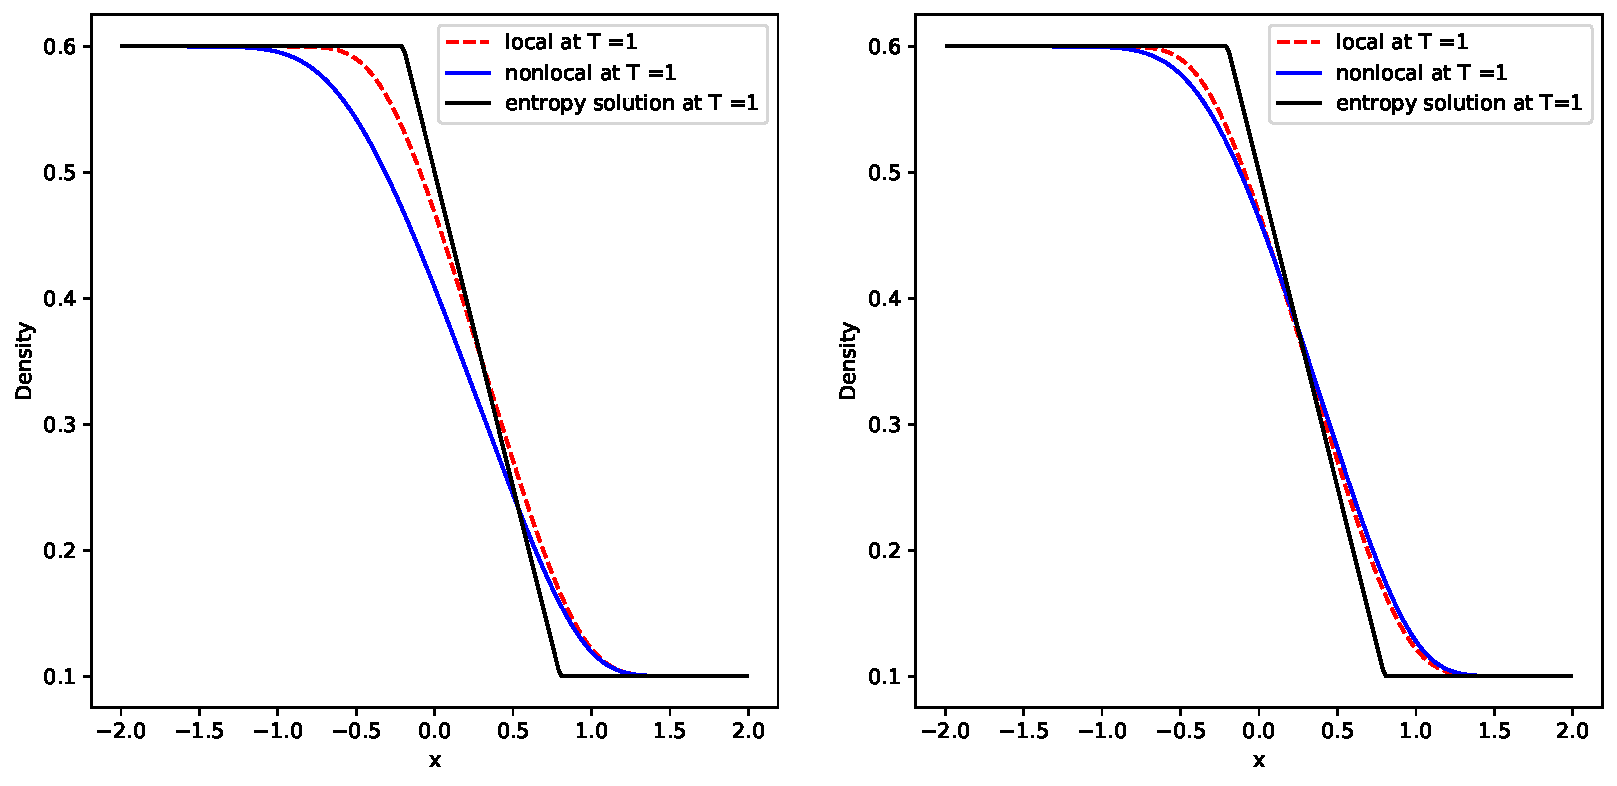
\includegraphics[width=\textwidth]{exp_1a.pdf}
    \caption{Numerical solutions and entropy solution at T = $1$ corresponding to the left endpoint numerical quadrature weights \eqref{eq:left_endpoint-quadrature} (left) and the normalized left endpoint numerical quadrature weights \eqref{eq:normalized_left_endpoint_quadrature}(right).}
    \label{fig:exp_1a}
\end{figure}
As shown in Figure~\ref{fig:exp_1a}, the choice of numerical quadrature weights does not lead to a significant difference between the numerical solutions and the entropy solution of the local model \eqref{eq:local model}. Nevertheless, a low level of accuracy remains at the shocks, where the numerical solutions deviate noticeably from the entropy solution. We aim to achieve convergence of the numerical solutions to the entropy solution as $\Delta x$ and $\epsilon$ tend to zero simultaneously.

\subsection*{Numerical Experiment 1b}
Next we choose $\epsilon = 0.01$ and $\Delta x = 0.005$

\begin{figure}[H]
    \centering
    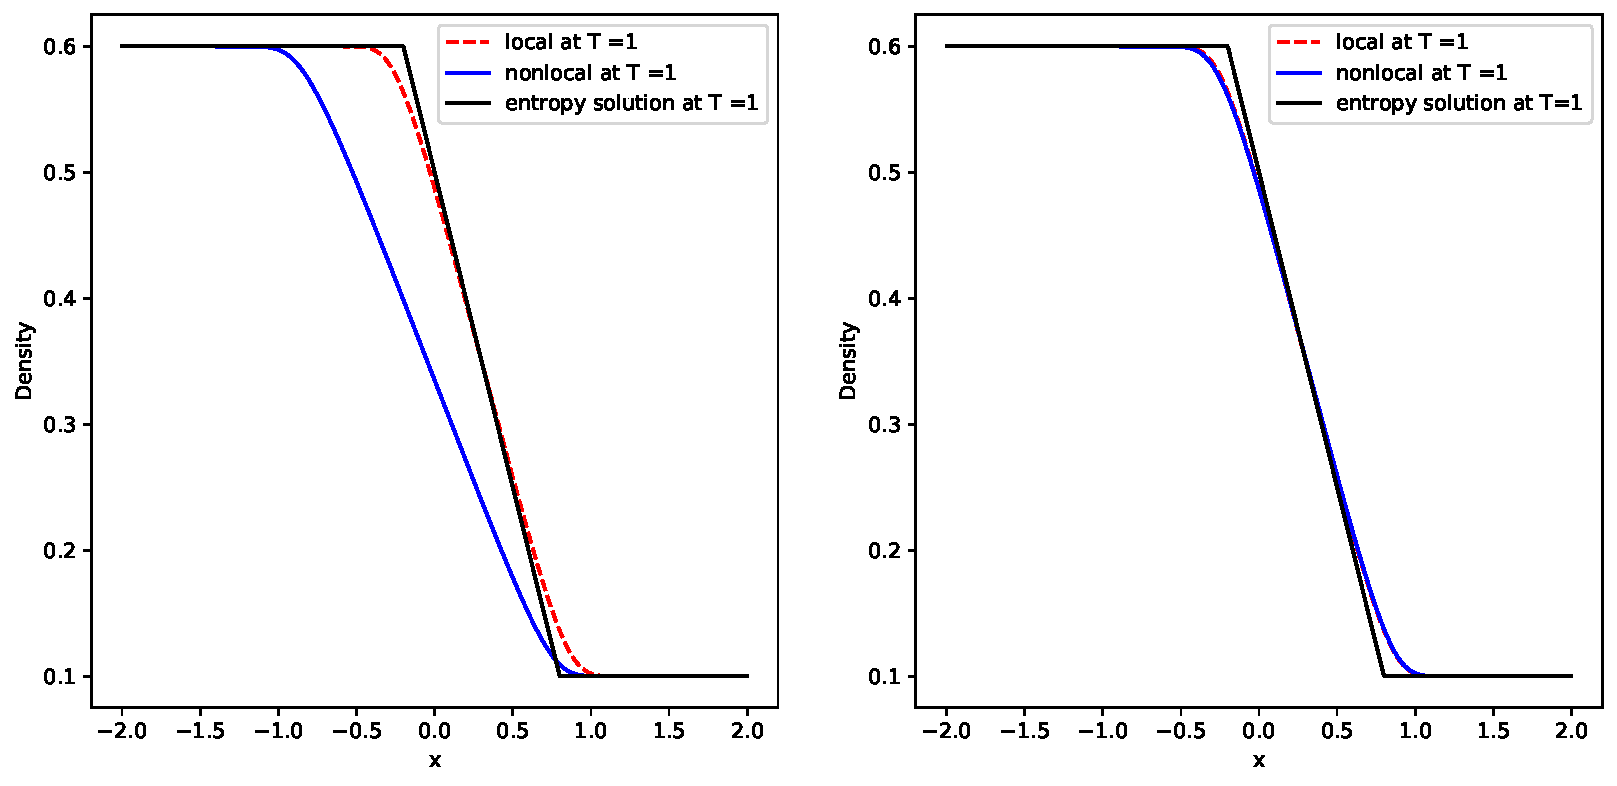
\includegraphics[width=\textwidth]{exp_1b.pdf}
    \caption{Numerical solutions and entropy solution at T = $1$ corresponding to the left endpoint numerical quadrature weights \eqref{eq:left_endpoint-quadrature} (left) and the normalized left endpoint numerical quadrature weights \eqref{eq:normalized_left_endpoint_quadrature} (right).}
    \label{fig:exp_1b}
\end{figure}
As observed in Figure~\ref{fig:exp_1b}, contrary to our expectations, the left endpoint numerical quadrature weights cause the numerical solution of the nonlocal model to deviate further from both the numerical solution and the entropy solution of the local model. In contrast, the normalized left endpoint quadrature weights lead to improved accuracy and better alignment between the numerical solutions and the entropy solution.

\subsection*{Numerical Experiment 1c}
Finally we take $\epsilon = 0.001$ and $\Delta x = 0.001$.
\begin{figure}[H]
    \centering
    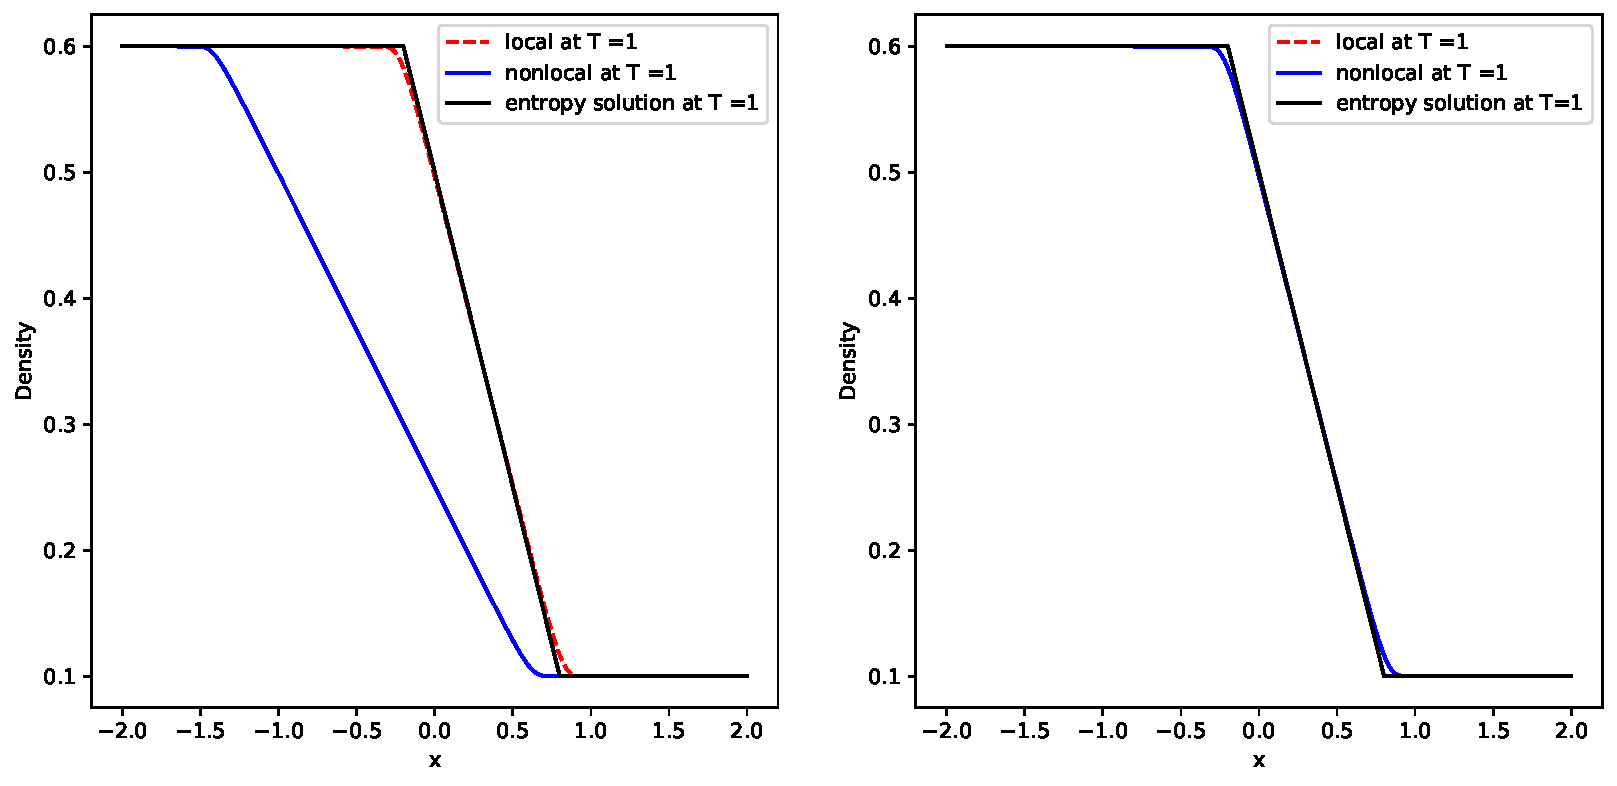
\includegraphics[width=\textwidth]{exp_1c.pdf}
    \caption{Numerical solutions and entropy solution at T = $1$ corresponding to the left endpoint numerical quadrature weights \eqref{eq:left_endpoint-quadrature} (left) and the normalized left endpoint numerical quadrature weights \eqref{eq:normalized_left_endpoint_quadrature} (right).}
    \label{fig:exp_1c}
\end{figure}
We observe in Figure~\ref{fig:exp_1c} that the numerical solution of the nonlocal model obtained using the left endpoint numerical quadrature weights completely fails. By contrast, significantly better accuracy is observed when using the normalized left endpoint numerical quadrature weights.
\subsection*{Summary}
The numerical experiments above demonstrate that, as $\Delta x$ and $\epsilon$ tend to zero simultaneously, while the Lax--Friedrichs type scheme based on the left endpoint quadrature weights becomes increasingly inaccurate, the normalized left endpoint quadrature weights consistently maintain stability and improved alignment with the entropy solution. The reason for this lies on the normalization condition, i.e, the sum of the numerical quadrature $w_k$ equals $1$. The above results provide evidence that the choice of numerical quadrature weights plays a crucial role in ensuring the asymptotic compatibility of the numerical method \eqref{eq:generic_H_N}.

\section{Numerical Convergence Analysis}\label{sec:Convergence_analysis}
The numerical experiments above indicate that the method \eqref{eq:generic_H_N} is consistent and stable when using the normalized left endpoint quadrature weights. We continue the numerical experiment to determine the convergence and order of convergence, and see if the Godunov numerical scheme\eqref{eq:God_F} is more accurate than the Lax--Friedrichs scheme \eqref{eq:Lax-F numerical flux}.
We are interested in presenting numerical experiments on whether:
\begin{itemize}
    \item $\rho^{\epsilon, \Delta x} \rightarrow u$ as both $\Delta x \rightarrow 0$ and $\epsilon \rightarrow 0$ simultaneously.
    \item $\rho^{\epsilon, \Delta x} \rightarrow \rho^{\epsilon}$ for fixed $\epsilon$ as $\Delta x \rightarrow 0$.
\end{itemize}

Considering the computed reference and numerical solutions as piecewise constant functions on each cell of size $\Delta x$, we measure the global error
\[
    e = U^{\mathrm{ref}} - U^{\mathrm{num}}
\]
using the $L^{1}$ norm:
\begin{align*}
    \| e \|_{L^{1}} = \Delta x \sum_{j=0}^{K-1} |e^j|.
\end{align*}
Here, $U^{\mathrm{ref}}$ and $U^{\mathrm{num}}$ denote the reference solution and the numerical solution, respectively. We aim to obtain
\[
    \| e \|_{L^{1}} \rightarrow 0
\]
as the parameters tend to zero.

\subsection{Numerical Convergence to the Local Model}
%\textcolor{red}{Rarefaction solution}
We will present the numerical experiments for $\rho^{\epsilon, \Delta x} \rightarrow u $ as both $\Delta x \rightarrow 0$ and $\epsilon \rightarrow 0$ simultaneously. In addition to the initial data \eqref{eq:sloving rarefaction} and \eqref{eq:sloving shocks}, we also consider the smooth initial data
\begin{equation}\label{eq:smooth}
    u(x,0) = 0.5 + 0.3\cos{\frac{\pi x}{2}}.
\end{equation}

We remember that, as described in Chapter~\ref{chap:chapter_2}, we have a formula for solving Riemann problems of the local model. Hence for the Riemann initial data \eqref{eq:sloving rarefaction} and \eqref{eq:sloving shocks} we take the corresponding reference solution $u$ to be the exact entropy solution given by \eqref{eq: u_L > u_R} and \eqref{eq: u_L < u_R}, respectively. For the smooth initial data \eqref{eq:smooth}, we compute the corresponding reference solution $u$ numerically on a fine grid for $\Delta x = \frac{4}{4096}$. With the relation $\epsilon = 3\Delta x$, we let both $\Delta x \rightarrow 0$ and \(\epsilon \to 0\) simultaneously, although $\Delta x = \frac{1}{2^{4+m}}$ for $m = 0,1,2,3, 4, 5,6$, and compute the $L^{1}$ errors and order of convergence.

Focusing on the initial data given in \eqref{eq:sloving rarefaction}, we plot the $L^{1}$ errors against the number of cells to compare the efficiency of the Godunov and Lax--Friedrichs scheme. We also present the observed order of convergence in Table~\ref{tab:table_1}
\begin{figure}[H]
    \centering
    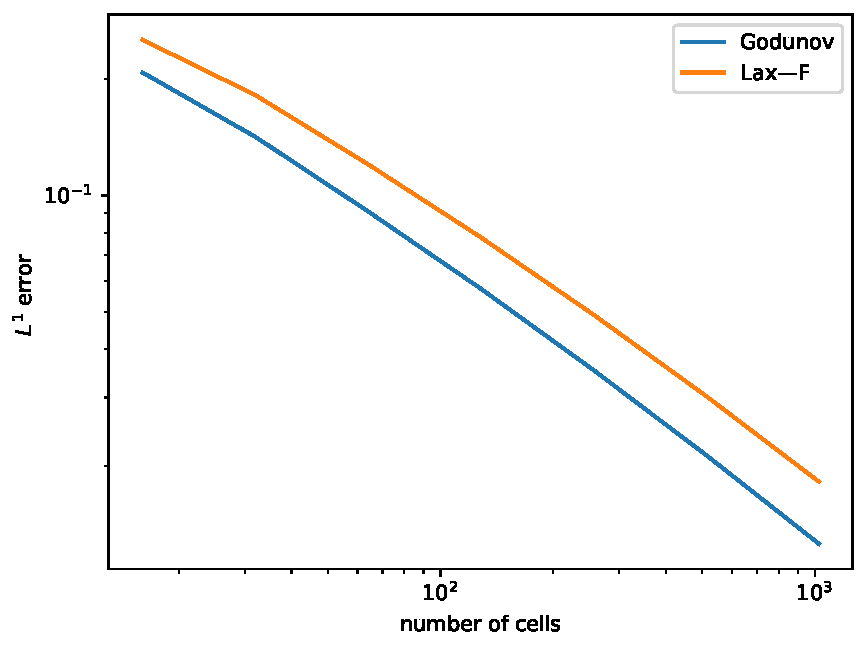
\includegraphics[width=0.7\textwidth]{Conver_local.pdf}
    \caption{$L^1$ error vs. number of cells}
    \label{fig:Conver_local_1}
\end{figure}
Figure~\ref{fig:Conver_local_1} indicates that the $L^{1}$-error for both Godunov and Lax--Friedrichs scheme tends to zero as the number of cells increases.
In other words, both the schemes converge to the unique entropy solution $u$ of the local model \eqref{eq:local model} as both \(\Delta x \to 0\) and \(\epsilon \to 0\) simultaneously. We observe as well that the Godunov scheme converges faster than Lax--Friedrichs scheme.
A natural question is: how fast do the schemes converge?
To answer this, we study the order of convergence $r$ for both schemes.

We assume that the $L^{1}$ error on a mesh of size $\Delta x_i$ can be written as
\begin{align*}
    E_i = C(\Delta x_i)^r,
\end{align*}
for some constant $C>0$.
If we have the error at two consecutive refinement levels $(E_{i-1},E_i)$, then we have
\begin{align*}
    \frac{E_{i-1}}{E_i}
    =\left(\frac{\Delta x_{i-1}}{\Delta x_i}\right)^{r}.
\end{align*}
Taking logarithms on both sides gives the standard expression for the order of convergence
\begin{align*}
    r =
    \frac{\log(E_{i-1}) - \log(E_i)}
    {\log(\Delta x_{i-1}) - \log(\Delta x_i)}.
\end{align*}
The order of convergence tells us how fast does a scheme converge to the correct solution, the higher order is the faster convergence.

\begin{table}[H]
    \centering
    \begin{minipage}{0.45\textwidth}
        \centering
        \begin{tabular}{ |p{1.5cm}||p{2.2cm}| |p{1.5cm}| }
            \hline
            \textbf{Cells } & $L^{1}$-\textbf{errors}  & \textbf{OOC} \\
            \hline
            16              & $2.5205 \times 10^{-1}$  & --           \\
            32              & $1.8141 \times 10^{-1}$  & 0.4744       \\
            64              & $1.2020 \times 10^{-1}$  & 0.5938       \\
            128             & $7.7851 \times 10^{-2}$  & 0.6267       \\
            256             & $4.9129 \times 10^{-2}$  & 0.6641       \\
            512             & $3.0257 \times 10^{-2}$  & 0.6993       \\
            1024            & $1.8184 \times 10^{-2} $ & 0.7346       \\
            \hline
        \end{tabular}
        \caption*{(a) Lax--Friedrichs scheme}
    \end{minipage}
    \hfill
    \begin{minipage}{0.5\textwidth}
        \centering
        \begin{tabular}{ |p{1.5cm}||p{2.2cm}| |p{1.5cm}| }
            \hline
            \textbf{Cells } & $L^{1}$-\textbf{errors} & \textbf{OOC} \\
            \hline
            16              & $2.0744 \times 10^{-1}$ & --           \\
            32              & $1.4154 \times 10^{-1}$ & 0.5515       \\
            64              & $9.0816 \times 10^{-2}$ & 0.6402       \\
            128             & $5.7350 \times 10^{-2}$ & 0.6632       \\
            256             & $3.5334 \times 10^{-2}$ & 0.6987       \\
            512             & $2.1299 \times 10^{-2}$ & 0.7303       \\
            1024            & $1.2565 \times 10^{-2}$ & 0.7614       \\
            \hline
        \end{tabular}
        \caption*{(b) Godunov scheme}
    \end{minipage}

    \caption{$L^{1}$-errors and observed order of convergence obtained using the Lax--Friedrichs scheme and the Godunov scheme in solving the local model with the Riemann initial data \eqref{eq:sloving rarefaction}.}
    \label{tab:table_1}
\end{table}
Table \ref{tab:table_1} presents the quantitative results for the $L^{1}$-errors and the observed order of convergence $r$ for the
Riemann initial data \eqref{eq:sloving rarefaction}, where $u_L > u_R$. We observe that the $L^{1}$-errors produced by the Godunov scheme are consistently smaller than those obtained using the Lax--Friedrichs scheme. For both schemes, the observed order of convergence is at most $1$, indicating relatively slow convergence.

Let us now consider the Riemann initial data \eqref{eq:sloving shocks}, where $u_L < u_R$.
We obtain the corresponding quantitative results:
\begin{table}[H]
    \centering
    \begin{minipage}{0.45\textwidth}
        \centering
        \begin{tabular}{ |p{1.5cm}||p{2.2cm}| |p{1.5cm}| }
            \hline
            \textbf{Cells } & $L^{1}$-\textbf{errors} & \textbf{OOC} \\
            \hline
            16              & $2.3182 \times 10^{-1}$ & --           \\
            32              & $1.4869 \times 10^{-1}$ & 0.6407       \\
            64              & $8.8979 \times 10^{-2}$ & 0.7408       \\
            128             & $5.0150 \times 10^{-2}$ & 0.8272       \\
            256             & $2.6012 \times 10^{-2}$ & 0.9470       \\
            512             & $1.3128 \times 10^{-2}$ & 0.9866       \\
            1024            & $6.5769 \times 10^{-3}$ & 0.9971       \\
            \hline
        \end{tabular}
        \caption*{(a) Lax--Friedrichs scheme}
    \end{minipage}
    \hfill
    \begin{minipage}{0.5\textwidth}
        \centering
        \begin{tabular}{ |p{1.5cm}||p{2.2cm}| |p{1.5cm}| }
            \hline
            \textbf{Cells } & $L^{1}$-\textbf{errors} & \textbf{OOC} \\
            \hline
            16              & $1.2876 \times 10^{-1}$ & --           \\
            32              & $8.5352 \times 10^{-2}$ & 0.5932       \\
            64              & $4.9126 \times 10^{-2}$ & 0.7969       \\
            128             & $2.6836 \times 10^{-2}$ & 0.8723       \\
            256             & $1.3336 \times 10^{-2}$ & 1.0089       \\
            512             & $6.7539 \times 10^{-3}$ & 0.9815       \\
            1024            & $3.3509 \times 10^{-3}$ & 1.0112       \\
            \hline
        \end{tabular}
        \caption*{(b) Godunov scheme}
    \end{minipage}
    \caption{$L^{1}$-errors and observed order of convergence obtained using the the Lax--Friedrichs scheme and the Godunov scheme in solving the local model with the Riemann initial data \eqref{eq:sloving shocks}}
    \label{tab:table_2}
\end{table}
The observation in Table \ref{tab:table_2} indicates that the Godunov numerical scheme handles solutions with shocks effectively than The Lax--Friedrichs scheme. We also observe that for both schemes the order of convergence is $1$.

Finally we repeat the above experiments with the smooth initial data \eqref{eq:smooth}, and obtain the corresponding quantitative results
\begin{table}[H]
    \centering
    \begin{minipage}{0.45\textwidth}
        \centering
        \begin{tabular}{ |p{1.5cm}||p{2.2cm}| |p{1.5cm}| }
            \hline
            \textbf{Cells } & $L^{1}$-\textbf{errors} & \textbf{OOC} \\
            \hline
            16              & $4.4055 \times 10^{-1}$ & --           \\
            32              & $2.7531 \times 10^{-1}$ & 0.6783       \\
            64              & $1.6123 \times 10^{-1}$ & 0.7719       \\
            128             & $9.0595 \times 10^{-2}$ & 0.8316       \\
            256             & $4.9132 \times 10^{-2}$ & 0.8828       \\
            512             & $2.5445 \times 10^{-2}$ & 0.9493       \\
            1024            & $1.2221 \times 10^{-2}$ & 1.0580       \\
            \hline
        \end{tabular}
        \caption*{(a) Lax--Friedrichs scheme}
    \end{minipage}
    \hfill
    \begin{minipage}{0.5\textwidth}
        \centering
        \begin{tabular}{ |p{1.5cm}||p{2.2cm}| |p{1.5cm}| }
            \hline
            \textbf{Cells } & $L^{1}$-\textbf{errors}  & \textbf{OOC} \\
            \hline
            16              & $3.1431 \times 10^{-1}$  & --           \\
            32              & $1.8983 \times 10^{-1}$  & 0.7275       \\
            64              & $1.0959 \times 10^{-1}$  & 0.7926       \\
            128             & $6.1083 \times 10^{-2}$  & 0.8433       \\
            256             & $3.3016 \times 10^{-2}$  & 0.8876       \\
            512             & $1.7172 \times 10^{-2}$  & 0.9432       \\
            1024            & $ 8.4201 \times 10^{-3}$ & 1.0281       \\
            \hline
        \end{tabular}
        \caption*{(b) Godunov scheme}
    \end{minipage}

    \caption{$L^{1}$-errors and observed order of convergence obtained using the the Lax--Friedrichs scheme and the Godunov scheme in solving the local model with smooth initial data \eqref{eq:smooth}.}
    \label{tab:table_3}
\end{table}
\subsection*{Summary}
The experiments above provide evidence that the numerical schemes are asymptotically compatible, in the sense that they converge to the entropy solution of the local model \eqref{eq:local model} as both parameters $\Delta x$ and $\epsilon$ tend to zero simultaneously. Moreover, although the stability analysis in Chapter~\ref{chap:chapter_4} is established under the assumption that the initial data can not contain negative jumps, the numerical experiments indicate that the methods remain robust even for the initial data \eqref{eq:sloving rarefaction}, which contains a negative jump.

\subsection{Numerical Convergence to the Nonlocal Model}

For fixed $\epsilon$, through numerical experiments we aim to deduce $ \| e \Vert_{L^{1}}= \| \rho^{\epsilon} - \rho^{\epsilon, \Delta x}\Vert_{L^{1}} \rightarrow 0$ as $\Delta x \rightarrow 0$. We compute the reference solution $\rho^{\epsilon}$ numerically for $\Delta x = \frac{4}{4096}$ and $\epsilon = 0.1$. Holding $\epsilon = 0.1$ fixed and letting $\Delta x \rightarrow 0$, although $\Delta x = \frac{1}{2^{4+m}}$ for $m = 0,1,2,3, 4, 5, 6$, we compute the $L^{1}$ errors and order of convergence.

%\begin{figure}[H]
%\centering
%
\includegraphics[width=0.7\textwidth]{Conver_2l.pdf}
%\caption{$L^1$ error vs. number of cells}
%\label{fig:Conver_1}
%\end{figure}

\begin{table}[H]
    \centering
    \begin{minipage}{0.45\textwidth}
        \centering
        \begin{tabular}{ |p{1.5cm}||p{2.2cm}| |p{1.5cm}| }
            \hline
            \textbf{Cells } & $L^{1}$-\textbf{errors}  & \textbf{OOC} \\
            \hline
            16              & $1.8626 \times 10^{-1}$  & --           \\
            32              & $1.2159 \times 10^{-1}$  & 0.6154       \\
            64              & $7.4547 \times 10^{-2}$  & 0.7058       \\
            128             & $ 4.2751 \times 10^{-2}$ & 0.8022       \\
            256             & $2.3350 \times 10^{-2}$  & 0.8725       \\
            512             & $1.1829 \times 10^{-2}$  & 0.9811       \\
            1024            & $5.3589 \times 10^{-3}$  & 1.1423       \\
            \hline
        \end{tabular}
        \caption*{(a) Lax--Friedrichs scheme}
    \end{minipage}
    \hfill
    \begin{minipage}{0.5\textwidth}
        \centering
        \begin{tabular}{ |p{1.5cm}||p{2.2cm}| |p{1.5cm}| }
            \hline
            \textbf{Cells } & $L^{1}$-\textbf{errors}  & \textbf{OOC} \\
            \hline
            16              & $1.2667 \times 10^{-1}$  & --           \\
            32              & $ 7.3044 \times 10^{-2}$ & 0.7942       \\
            64              & $4.2832 \times 10^{-2}$  & 0.7701       \\
            128             & $2.3189 \times 10^{-2}$  & 0.8853       \\
            256             & $1.2184 \times 10^{-2}$  & 0.9285       \\
            512             & $5.9654 \times 10^{-3}$  & 1.0303       \\
            1024            & $ 2.6423 \times 10^{-3}$ & 1.1748       \\
            \hline
        \end{tabular}
        \caption*{(b) Godunov scheme}
    \end{minipage}

    \caption{$L^{1}$-errors and observed order of convergence obtained using the the Lax--Friedrichs scheme and the Godunov scheme in solving the nonlocal model with the Riemann initial data \eqref{eq:sloving rarefaction}.}
    \label{tab:table_4}
\end{table}

\begin{table}[H]
    \centering
    \begin{minipage}{0.45\textwidth}
        \centering
        \begin{tabular}{ |p{1.5cm}||p{2.2cm}| |p{1.5cm}| }
            \hline
            \textbf{Cells } & $L^{1}$-\textbf{errors} & \textbf{OOC} \\
            \hline
            16              & $2.0628 \times 10^{-1}$ & --           \\
            32              & $1.0767 \times 10^{-1}$ & 0.9380       \\
            64              & $7.1225 \times 10^{-2}$ & 0.5962       \\
            128             & $3.8519 \times 10^{-2}$ & 0.8868       \\
            256             & $2.0491 \times 10^{-2}$ & 0.9106       \\
            512             & $1.0478 \times 10^{-2}$ & 0.9676       \\
            1024            & $4.8977 \times 10^{-3}$ & 1.0972       \\
            \hline
        \end{tabular}
        \caption*{(a) Lax--Friedrichs scheme}
    \end{minipage}
    \hfill
    \begin{minipage}{0.5\textwidth}
        \centering
        \begin{tabular}{ |p{1.5cm}||p{2.2cm}| |p{1.5cm}| }
            \hline
            \textbf{Cells } & $L^{1}$-\textbf{errors} & \textbf{OOC} \\
            \hline
            16              & $1.0844 \times 10^{-1}$ & --           \\
            32              & $4.4663 \times 10^{-2}$ & 1.2798       \\
            64              & $3.3717 \times 10^{-2}$ & 0.4056       \\
            128             & $1.6571 \times 10^{-2}$ & 1.0248       \\
            256             & $8.2085 \times 10^{-3}$ & 1.0134       \\
            512             & $3.9258 \times 10^{-3}$ & 1.0641       \\
            1024            & $1.7225 \times 10^{-3}$ & 1.1885       \\
            \hline
        \end{tabular}
        \caption*{(b) Godunov scheme}
    \end{minipage}

    \caption{$L^{1}$-errors and observed order of convergence obtained using the the Lax--Friedrichs scheme and the Godunov scheme in solving the nonlocal model with the Riemann initial data \eqref{eq:sloving shocks}}
    \label{tab:table_5}
\end{table}


\begin{table}[H]
    \centering
    \begin{minipage}{0.45\textwidth}
        \centering
        \begin{tabular}{ |p{1.5cm}||p{2.2cm}| |p{1.5cm}| }
            \hline
            \textbf{Cells } & $L^{1}$-\textbf{errors}  & \textbf{OOC} \\
            \hline
            16              & $3.3092 \times 10^{-1}$  & --           \\
            32              & $1.8065 \times 10^{-1} $ & 0.8733       \\
            64              & $9.9861 \times 10^{-2} $ & 0.8552       \\
            128             & $5.2189 \times 10^{-2}$  & 0.9362       \\
            256             & $2.6458 \times 10^{-2}$  & 0.9801       \\
            512             & $1.2647 \times 10^{-2}$  & 1.0649       \\
            1024            & $ 5.5133 \times 10^{-3}$ & 1.1978       \\
            \hline
        \end{tabular}
        \caption*{(a) Lax--Friedrichs scheme}
    \end{minipage}
    \hfill
    \begin{minipage}{0.5\textwidth}
        \centering
        \begin{tabular}{ |p{1.5cm}||p{2.2cm}| |p{1.5cm}| }
            \hline
            \textbf{Cells } & $L^{1}$-\textbf{errors} & \textbf{OOC} \\
            \hline
            16              & $1.8322 \times 10^{-1}$ & --           \\
            32              & $8.6063 \times 10^{-2}$ & 1.0901       \\
            64              & $4.5197 \times 10^{-2}$ & 0.9291       \\
            128             & $2.2487 \times 10^{-2}$ & 1.0071       \\
            256             & $1.1061 \times 10^{-2}$ & 1.0237       \\
            512             & $5.1421 \times 10^{-3}$ & 1.1050       \\
            1024            & $2.2161 \times 10^{-3}$ & 1.2143       \\
            \hline
        \end{tabular}
        \caption*{(b) Godunov scheme}
    \end{minipage}

    \caption{$L^{1}$-errors and observed order of convergence obtained using the the Lax--Friedrichs scheme and the Godunov scheme in solving the nonlocal model with the smooth initial data \eqref{eq:smooth}.}
    \label{tab:table_6}
\end{table}
\subsection*{Summary}
The quantitative results above indicate that for fixed $\epsilon$, $\rho^{\epsilon, \Delta x} \rightarrow \rho^{\epsilon} $ as $\Delta x \rightarrow 0$. In addition, the Godunov scheme is more efficient than the Lax--Friedrichs scheme. In addition, based on our numerical experiments, the order of the developed numerical schemes is at most $1$. So, in the next chapter we will develop a second-oder numerical scheme.




\section{A Second order Numerical Scheme}
\subsection{Semidiscrete Formulation}
The integral form of the conservation law we stated in section 3 is suitable for first order accurate schemes. In order to drive higher order schemes, we need a more flexible formulation which is called a semidiscrete formulation. This formulation allows us to separately increase the order of spatial and temporal accuracy, see \textcolor{red}{Citation needed here}.

Taking now each cell average over $C_j$ to be given by
\begin{equation}
    \begin{split}
        u_j(t) = \frac{1}{\Delta x}\int_{x_{j-\sfrac{1}{2}}}^{x_{j+\sfrac{1}{2}}} u(x,t) \,dx
    \end{split}
\end{equation}
and integrating \eqref{eq:local model} over the domain $C_j$
\begin{align*}
    \int_{x_{j-\sfrac{1}{2}}}^{x_{j+\sfrac{1}{2}}} u_{t} + f(u)_{x} \,dx  = 0
\end{align*}
gives us
\[
    \frac{d}{dt}u_j(t) + \sfrac{1}{\Delta x}\Bigl(f(u(x_{j+\sfrac12}^{-},t))- f(u(x_{j-\sfrac12}^{+},t))\Bigr)
\]
where
\[
    u(x_{j+\sfrac12}^{-},t) = \lim_{x\rightarrow x_{j+\sfrac12}^{-}} u(x,t)\]
and
\[
    u(x_{j+\sfrac12}^{+},t) = \lim_{x\rightarrow x_{j+\sfrac12}^{+}} u(x,t)
\]
denotes the left and right-limit of $u$ at $x_{j+\sfrac12}$, respectively.

Let $F$ be an approximation of the fluxes such that,
\[
    F_{j+\sfrac12}^{\pm} \approx f(u(x_{j+\sfrac12}^{\pm},t)),
\]
then we obtain the semidiscrete formulation as
\begin{equation}\label{eq:semidiscrete}
    \begin{cases}
        \frac{d}{dt}u_j(t) + \frac{1}{\Delta x}\Bigl(F_{j+\frac12}^{-}- F_{j-\frac12}^{+}\Bigr) = 0 \\[2ex]
        u_j(0)= \int_{x_{j-\sfrac12}}^{x_{j+\sfrac12}} u_0{x} \, dx
    \end{cases}
\end{equation}
Which is a system of ODEs that must be integrated in time by a suitable time integration
routine.
\subsection{Second Order Semidiscrete Scheme}
Having the semidiscrete formulation \eqref{eq:semidiscrete}, we can now separately increase
the order of spatial and temporal accuracy. We observe in the formulation above that we need the edge values $u_j^{\pm} = u(x_{j +\sfrac{1}{2}}^\pm,t)$. If we let the edge values to be piecewise constants in space and apply a forward Euler time integration, we obtain the standard first-order finite volume scheme. In order to obtain a second-order finite volume scheme, we need to construct a linear piecewise function in each cell, so the edge values are evaluated on the reconstructed functions.

Given a cell average $u_j^{n}$ of $C_j$ at time $t^n$, we can construct a linear function
\[
    \bar{u}_j(x)= u_j^{n} + \sigma_j \frac{x-x_j}{\Delta x}, \quad x \in C_j
\]
where the slope $\sigma_j$ is selected, such that $\bar{u}_j(x)$ is conservative and satisfy the TVD property.

We choose the slope by the minmod limiter
\[
    \sigma_j^n
    =
    minmod\!\left(
    u_j^n-u_{j-1}^n,\,
    \frac12(u_{j+1}^n-u_{j-1}^n),\,
    u_{j+1}^n-u_j^n
    \right).
\]
Here
\[
    minmod(a_1,\dots,a_m)
    =
    \begin{cases}
        \operatorname{sgn}(a_1)\min_{1\leq \ell\leq m}|a_\ell|,
           & \text{if } \operatorname{sgn}(a_1)=\cdots=\operatorname{sgn}(a_m), \\[1mm]
        0, & \text{otherwise}.
    \end{cases}
\]
We can now use $\bar{u}_j$ to approximate $u(x_{j+\sfrac12}^{-},t)$ and $u(x_{j+\sfrac12}^{+},t)$, such that the left and right-limit values are given by
\begin{align*}
    u_{j+\frac12}^- & := \lim_{x\rightarrow x_{j+\sfrac12}^{-}} \bar{u}_j(x) \\
                    & =u_j^n+\frac12\sigma_j^n
\end{align*}
and
\begin{align*}
    u_{j+\frac12}^+ & := \lim_{x\rightarrow x_{j+\sfrac12}^{+}} \bar{u}_j(x) \\
                    & =u_{j+1}^n-\frac12\sigma_{j+1}^n
\end{align*}
In section $3$ we approximated the convolution term
\[
    \int_{0}^{\epsilon} \omega_{\epsilon}(y) u(x+y,t) \, dy
\]
using piecewise constants, which led us to the first-order finite volume scheme. In order to obtain the second-order finite volume scheme, we approximate the convolution term using the piecewise linear function $\bar{u}(x,t)= \bar{u}_j(x)$ for $x \in C_j$ and trapezoidal rule as following:\\
Following the approach in \textcolor{red}{Citation needed here}, we assume that the function $\omega_{\epsilon}$ is a convolution kernel with compact support in $[0,\epsilon]$.\\
let
\[M:=\lceil \frac{\epsilon}{\Delta x}\rceil,  \]
and
\[
    I_{j+\sfrac12}:= \int_{0}^{\epsilon} \omega_{\epsilon}(y) u(x_{j+\sfrac12}+y,t) \, dy.
\]
We apply first $\bar{u}$ such that $u(x_{j+\sfrac12}+y,t) \approx \bar{u}(x_{j+\sfrac12}+y,t)$ to get
\[
    I_{j+\sfrac12} \approx \int_{0}^{\epsilon} \omega_{\epsilon}(y) \bar{u}(x_{j+\sfrac12}+y,t) \, dy \\
\]
\[
    =\sum_{k=0}^{M-1} \int_{k\Delta x}^{(k+1)\Delta x} \omega_{\epsilon}(y) \bar{u}(x_{j+\sfrac12}+y,t) \, dy.
\]
We can now apply the trapezoidal rule to get
\begin{align*}
    I_{j+\sfrac12} & \approx \frac{\Delta x}{2}\sum_{k=0}^{M-1} \Bigl(\omega_{\epsilon}(k\Delta x)\bar{u}(x_{j+\sfrac12}+k\Delta x,t) + \omega_{\epsilon}((k+1)\Delta x)\bar{u}(x_{j+\sfrac12}+(k+1)\Delta x,t)\Bigr) \\
                   & = \frac{\Delta x}{2} \sum_{k=0}^{M-1} \Bigl(\omega_{\epsilon}(k\Delta x)\bar{u}(x_{j+k+\sfrac12},t) + \omega_{\epsilon}((k+1)\Delta x)\bar{u}(x_{j+k+1+\sfrac12},t) \Bigr)                       \\
                   & = \frac{\Delta x}{2}\sum_{k=0}^{M-1} \Bigl(w_k \bar{u}(x_{j+k+\sfrac12},t) + w_{k+1}\bar{u}(x_{j+k+\sfrac32},t) \Bigr)                                                                           \\
                   & = \frac{\Delta x}{2}\sum_{k=0}^{M-1} \Bigl( w_k u_{j+k+\sfrac12}^+ + w_{k+1}u_{j+k+\sfrac32}^- \Bigr)                                                                                            \\
\end{align*}
where $w_k$ is the left end point numerical quadrature denoted by
\[ w_k = \omega_{\epsilon}(k\Delta x), \qquad k = 0, \cdots M\]
We have seen in section $3$ that the normalization of the numerical quadrature plays essential role in consistency between the local and nonlocal model. Hence normalization is needed here as well.\\
Define
\[
    Q_{\Delta x}:= \frac{\Delta x}{2} \sum_{k=0}^{M-1} \Bigl( w_k + w_{k+1}\Bigr), \qquad \tilde{w}_k:= \frac{w_k}{Q_{\Delta x}}, \qquad k = 0, \cdots M
\]
So the normalization condition is satisfied, in the sense
\[\frac{\Delta x}{2} \sum_{k=0}^{M-1} \Bigl( \tilde{w}_k + \tilde{w}_{k+1}\Bigr) = 1. \]
If we now replace $w_k$ by $\tilde{w}_k$ in
\[ R_{j+\sfrac12}= \frac{\Delta x}{2} \sum_{k=0}^{M-1} \Bigl( w_k u_{j+k+\sfrac12}^+ + w_{k+1}u_{j+k+\sfrac32}^- \Bigr),\]
we get the approximation of the convolution term
\[ R_{j+\sfrac12}= \frac{\Delta x}{2} \sum_{k=0}^{M-1} \Bigl( \tilde{w}_k u_{j+k+\sfrac12}^+ + \tilde{w}_{k+1}u_{j+k+\sfrac32}^- \Bigr). \]
Letting the numerical flux $F_{j+\sfrac12}^-$ in \eqref{eq:semidiscrete} be defined by the Godunov-type flux
\[
    F_{j+\sfrac12}^- := u_{j+\sfrac12}^-(1-R_{j+\sfrac12}),
\]
and denoting
\[
    L_{\epsilon}(u)_j = \frac{1}{\Delta x} ( F_{j+\sfrac12}^- - F_{j-\sfrac12}^+ ),
\]
we obtain the semidiscrete nonlocal scheme:
\begin{equation}\label{eq:nonlocal-semidiscrete}
    \begin{cases}
        \frac{d}{dt}u_j(t) + L_{\epsilon}(u)_j = 0 \\[2ex]
        u_j(0)= \int_{x_{j-\sfrac12}}^{x_{j+\sfrac12}} u_0{x} \, dx
    \end{cases}
\end{equation}
\begin{proposition}
    Let $\Delta x > 0$. Then, as $\varepsilon \to 0$, the nonlocal semidiscrete scheme
    \eqref{eq:nonlocal-semidiscrete} converges to the local semidiscrete scheme
    \begin{equation}\label{eq:local-semidiscrete}
        \begin{cases}
            \displaystyle
            \frac{d}{dt} u_j(t) + L(u)_j = 0, \\[2ex]
            \displaystyle
            u_j(0) = \int_{x_{j-\sfrac12}}^{x_{j+\sfrac12}} u_0(x)\, dx,
        \end{cases}
    \end{equation}
    where
    \[
        L(u)_j := \frac{1}{\Delta x}
        \bigl(G_{j+\sfrac12}^- - G_{j-\sfrac12}^+ \bigr) ,\qquad G_{j+\sfrac12}^- := u_{j+\sfrac12}^-(1 - u_{j+\sfrac12}^+)
    \]
\end{proposition}
\subsection{Comparison of First Order and Second Order Godunov Scheme}
\subsection{Numerical Convergence to the Nonlocal Model}
\textcolor{red}{Rarefaction solution}
\begin{table}[H]
    \centering
    \begin{minipage}{0.45\textwidth}
        \centering
        \begin{tabular}{ |p{1.5cm}||p{2cm}| |p{1.5cm}| }
            \hline
            \textbf{Cells } & $L^{1}$-\textbf{errors}  & \textbf{OOC} \\
            \hline
            16              & $1.2667 \times 10^{-1}$  & --           \\
            32              & $7.3044 \times 10^{-2}$  & 0.7942       \\
            64              & $4.2832 \times 10^{-2}$  & 0.7701       \\
            128             & $ 2.3189 \times 10^{-2}$ & 0.8853       \\
            256             & $1.2184 \times 10^{-2}$  & 0.9285       \\
            512             & $5.9654 \times 10^{-3}$  & 1.0303       \\
            1024            & $ 2.6423 \times 10^{-3}$ & 1.1748       \\
            \hline
        \end{tabular}
        \caption*{(a) First order Godunov scheme}
    \end{minipage}
    \hfill
    \begin{minipage}{0.5\textwidth}
        \centering
        \begin{tabular}{ |p{1.5cm}||p{2cm}| |p{1.5cm}| }
            \hline
            \textbf{Cells } & $L^{1}$-\textbf{errors}  & \textbf{OOC} \\
            \hline
            16              & $5.0110 \times 10^{-2}$  & --           \\
            32              & $1.7309 \times 10^{-2}$  & 1.5336       \\
            64              & $7.9544 \times 10^{-3}$  & 1.1217       \\
            128             & $3.0467 \times 10^{-3}$  & 1.3845       \\
            256             & $1.4243 \times 10^{-3}$  & 1.0971       \\
            512             & $6.5964 \times 10^{-4}$  & 1.1104       \\
            1024            & $ 2.9541 \times 10^{-4}$ & 1.1590       \\
            \hline
        \end{tabular}
        \caption*{(b) Second order Godunov scheme}
    \end{minipage}

    \caption{$L^{1}$-errors and observed order of convergence obtained using the the Godunov first and second order scheme in solving the nonlocal model with the Riemann initial data \eqref{eq:sloving rarefaction}.}
    \label{tab:table 7}
\end{table}
\hrulefill \\
\textcolor{red}{Discontinuous solution}
\begin{table}[H]
    \centering
    \begin{minipage}{0.45\textwidth}
        \centering
        \begin{tabular}{ |p{1.5cm}||p{2cm}| |p{1.5cm}| }
            \hline
            \textbf{Cells } & $L^{1}$-\textbf{errors} & \textbf{OOC} \\
            \hline
            16              & $1.0844 \times 10^{-1}$ & --           \\
            32              & $4.4663 \times 10^{-2}$ & 1.2798       \\
            64              & $3.3717 \times 10^{-2}$ & 0.4056       \\
            128             & $1.6571 \times 10^{-2}$ & 1.0248       \\
            256             & $8.2085 \times 10^{-3}$ & 1.0134       \\
            512             & $3.9258 \times 10^{-3}$ & 1.0641       \\
            1024            & $1.7225 \times 10^{-3}$ & 1.1885       \\
            \hline
        \end{tabular}
        \caption*{(a) First order Godunov scheme}
    \end{minipage}
    \hfill
    \begin{minipage}{0.5\textwidth}
        \centering
        \begin{tabular}{ |p{1.5cm}||p{2cm}| |p{1.5cm}| }
            \hline
            \textbf{Cells } & $L^{1}$-\textbf{errors}  & \textbf{OOC} \\
            \hline
            16              & $7.1040 \times 10^{-2}$  & --           \\
            32              & $ 1.8091 \times 10^{-2}$ & 1.9734       \\
            64              & $1.5403 \times 10^{-2}$  & 0.2321       \\
            128             & $5.7654 \times 10^{-3}$  & 1.4177       \\
            256             & $1.9766 \times 10^{-3}$  & 1.5444       \\
            512             & $5.6019 \times 10^{-4}$  & 1.8190       \\
            1024            & $1.4551 \times 10^{-4}$  & 1.9448       \\
            \hline
        \end{tabular}
        \caption*{(b) Second order Godunov scheme}
    \end{minipage}

    \caption{$L^{1}$-errors and observed order of convergence obtained using the the Godunov first and second order scheme in solving the nonlocal model with with the Riemann initial data $u_L = 0.1 < 0.6= u_R$.}
    \label{tab:table 8}
\end{table}

\hrulefill \\
\qquad \textcolor{red}{Smooth solution}
\begin{table}[H]
    \centering
    \begin{minipage}{0.45\textwidth}
        \centering
        \begin{tabular}{ |p{1.5cm}||p{2cm}| |p{1.5cm}| }
            \hline
            \textbf{Cells } & $L^{1}$-\textbf{errors} & \textbf{OOC} \\
            \hline
            16              & $1.8322 \times 10^{-1}$ & --           \\
            32              & $8.6063 \times 10^{-2}$ & 1.0901       \\
            64              & $4.5197 \times 10^{-2}$ & 0.9291       \\
            128             & $2.2487 \times 10^{-2}$ & 1.0071       \\
            256             & $1.1061 \times 10^{-2}$ & 1.0237       \\
            512             & $5.1421 \times 10^{-3}$ & 1.1050       \\
            1024            & $2.2161 \times 10^{-3}$ & 1.2143       \\
            \hline
        \end{tabular}
        \caption*{(a) First order Godunov scheme}
    \end{minipage}
    \hfill
    \begin{minipage}{0.5\textwidth}
        \centering
        \begin{tabular}{ |p{1.5cm}||p{2cm}| |p{1.5cm}| }
            \hline
            \textbf{Cells } & $L^{1}$-\textbf{errors}  & \textbf{OOC} \\
            \hline
            16              & $7.5224 \times 10^{-2}$  & --           \\
            32              & $2.2102 \times 10^{-2}$  & 1.7670       \\
            64              & $6.3384 \times 10^{-3} $ & 1.8020       \\
            128             & $2.1914 \times 10^{-3}$  & 1.5322       \\
            256             & $4.8969 \times 10^{-4}$  & 2.1619       \\
            512             & $1.5326 \times 10^{-4}$  & 1.6759       \\
            1024            & $3.0656 \times 10^{-5}$  & 2.3218       \\
            \hline
        \end{tabular}
        \caption*{(b) Second order Godunov scheme}
    \end{minipage}

    \caption{$L^{1}$-errors and observed order of convergence obtained using the the Godunov first and second order scheme in solving the nonlocal model with the smooth initial data \eqref{eq:smooth}.}
    \label{tab:table 9}
\end{table}
\subsection{Numerical Convergence to the local Model}
\textcolor{red}{Rarefaction solution}
\begin{table}[H]
    \centering
    \begin{minipage}{0.45\textwidth}
        \centering
        \begin{tabular}{ |p{1.5cm}||p{2cm}| |p{1.5cm}| }
            \hline
            \textbf{Cells } & $L^{1}$-\textbf{errors} & \textbf{OOC} \\
            \hline
            16              & $2.0744 \times 10^{-1}$ & --           \\
            32              & $1.4154 \times 10^{-1}$ & 0.5515       \\
            64              & $9.0816 \times 10^{-2}$ & 0.6402       \\
            128             & $5.7350 \times 10^{-2}$ & 0.6632       \\
            256             & $3.5334 \times 10^{-2}$ & 0.6987       \\
            512             & $2.1299 \times 10^{-2}$ & 0.7303       \\
            1024            & $1.2565 \times 10^{-2}$ & 0.7614       \\
            \hline
        \end{tabular}
        \caption*{(a) First order Godunov scheme}
    \end{minipage}
    \hfill
    \begin{minipage}{0.5\textwidth}
        \centering
        \begin{tabular}{ |p{1.5cm}||p{2cm}| |p{1.5cm}| }
            \hline
            \textbf{Cells } & $L^{1}$-\textbf{errors}  & \textbf{OOC} \\
            \hline
            16              & $1.6004 \times 10^{-1}$  & --           \\
            32              & $1.0047 \times 10^{-1}$  & 0.6717       \\
            64              & $6.1193 \times 10^{-2} $ & 0.7153       \\
            128             & $3.6977 \times 10^{-2}$  & 0.7267       \\
            256             & $2.1940 \times 10^{-2}$  & 0.7530       \\
            512             & $1.2857 \times 10^{-2} $ & 0.7711       \\
            1024            & $7.4261 \times 10^{-3} $ & 0.7918       \\
            \hline
        \end{tabular}
        \caption*{(b) Second order Godunov scheme}
    \end{minipage}

    \caption{$L^{1}$-errors and observed order of convergence obtained using the the Godunov first and second order scheme in solving the local model with the Riemann initial data \eqref{eq:sloving rarefaction}.}
    \label{tab:table 10}
\end{table}

\hrulefill \\
\textcolor{red}{Discontinuous solution}
\begin{table}[H]
    \centering
    \begin{minipage}{0.45\textwidth}
        \centering
        \begin{tabular}{ |p{1.5cm}||p{2cm}| |p{1.5cm}| }
            \hline
            \textbf{Cells } & $L^{1}$-\textbf{errors} & \textbf{OOC} \\
            \hline
            16              & $1.2876 \times 10^{-1}$ & --           \\
            32              & $8.5352 \times 10^{-2}$ & 0.5932       \\
            64              & $4.9126 \times 10^{-2}$ & 0.7969       \\
            128             & $2.6836 \times 10^{-2}$ & 0.8723       \\
            256             & $1.3336 \times 10^{-2}$ & 1.0089       \\
            512             & $6.7539 \times 10^{-3}$ & 0.9815       \\
            1024            & $3.3509 \times 10^{-3}$ & 1.0112       \\
            \hline
        \end{tabular}
        \caption*{(a) First order Godunov scheme}
    \end{minipage}
    \hfill
    \begin{minipage}{0.5\textwidth}
        \centering
        \begin{tabular}{ |p{1.5cm}||p{2cm}| |p{1.5cm}| }
            \hline
            \textbf{Cells } & $L^{1}$-\textbf{errors} & \textbf{OOC} \\
            \hline
            16              & $9.8507 \times 10^{-2}$ & --           \\
            32              & $6.1071 \times 10^{-2}$ & 0.6897       \\
            64              & $2.9665 \times 10^{-2}$ & 1.0417       \\
            128             & $1.5514 \times 10^{-2}$ & 0.9352       \\
            256             & $7.7374 \times 10^{-3}$ & 1.0036       \\
            512             & $4.0784 \times 10^{-3}$ & 0.9238       \\
            1024            & $1.8805 \times 10^{-3}$ & 1.1169       \\
            \hline
        \end{tabular}
        \caption*{(b) Second order Godunov scheme}
    \end{minipage}

    \caption{$L^{1}$-errors and observed order of convergence obtained using the the Godunov first and second order scheme in solving the local model with with the Riemann initial data $u_L = 0.1 < 0.6= u_R$.}
    \label{tab:table 11}
\end{table}

\hrulefill \\
\qquad \textcolor{red}{Smooth solution}
\begin{table}[H]
    \centering
    \begin{minipage}{0.45\textwidth}
        \centering
        \begin{tabular}{ |p{1.5cm}||p{2cm}| |p{1.5cm}| }
            \hline
            \textbf{Cells } & $L^{1}$-\textbf{errors} & \textbf{OOC} \\
            \hline
            16              & $3.1430 \times 10^{-1}$ & --           \\
            32              & $1.8983 \times 10^{-1}$ & 0.7275       \\
            64              & $1.0959 \times 10^{-1}$ & 0.7926       \\
            128             & $6.1083 \times 10^{-2}$ & 0.8433       \\
            256             & $3.3015 \times 10^{-2}$ & 0.8876       \\
            512             & $1.7170 \times 10^{-2}$ & 0.9432       \\
            1024            & $8.4186 \times 10^{-3}$ & 1.0283       \\
            \hline
            \hline
        \end{tabular}
        \caption*{(a) First order Godunov scheme}
    \end{minipage}
    \hfill
    \begin{minipage}{0.5\textwidth}
        \centering
        \begin{tabular}{ |p{1.5cm}||p{2cm}| |p{1.5cm}| }
            \hline
            \textbf{Cells } & $L^{1}$-\textbf{errors}  & \textbf{OOC} \\
            \hline
            16              & $2.3215 \times 10^{-1}$  & --           \\
            32              & $1.3042 \times 10^{-1}$  & 0.8319       \\
            64              & $7.2110 \times 10^{-2}$  & 0.8549       \\
            128             & $ 3.9305 \times 10^{-2}$ & 0.8755       \\
            256             & $2.1099 \times 10^{-2}$  & 0.8975       \\
            512             & $1.1225 \times 10^{-2}$  & 0.9104       \\
            1024            & $5.8947 \times 10^{-3} $ & 0.9292       \\
            \hline
        \end{tabular}
        \caption*{(b) Second order Godunov scheme}
    \end{minipage}

    \caption{$L^{1}$-errors and observed order of convergence obtained using the the Godunov first and second order scheme in solving the local model with the smooth initial data \eqref{eq:smooth}.}
    \label{tab:table 12}
\end{table}


%\section{ Checking if H is Monotone}




As the $\lambda(r_j^n)^2$ is nonnegative and $\sum_{k=-1}^m c_{j,k}^n = 1$, it remains to show that $c_{j,k}^n \geq 0$ for all $k= -1, 0,1, \cdots, m.$

Clearly, $c_{j,-1}^n \geq 0$ because we have shown that in \eqref{eq:First_argument}
\begin{align*}
    c_{j,-1}^n & =\frac{\partial \mathcal{H}}{\partial \rho_{j-1}^n}              \\
               & = \lambda(1-q_j^n) \geq 0 \qquad \text{as } 0 \leq q_j^n \leq 1.
\end{align*}
For $k= 0$, we have
\begin{align*}
    c_{j,0}^n & = 1 - \lambda (1- q_j^n) + \lambda p_{j,0}^n -2\lambda r_j^n                            \\
              & = 1 - \lambda (1- q_j^n) + \lambda \Bigl(-w_0\rho_j^n + w_0 r_j^n\Bigr) -2\lambda r_j^n \\
              & = 1- \lambda \Bigl[(1- q_j^n)+ w_0\rho_j^n  + (2-w_0)r_j^n\Bigr]
\end{align*}
In order to have  $c_{j,0}^n \geq 0$, it holds to show that $\lambda \Bigl[(1- q_j^n)+ w_0\rho_j^n  + (2-w_0)r_j^n\Bigr] \leq 1$. But by \eqref{eq:lambda_God} we have $\lambda < \frac{1}{2}$. Therefore, it is sufficient to show that
\[
    (1- q_j^n)+ w_0\rho_j^n  + (2-w_0)r_j^n \leq 2.
\]
Mark that all the terms $(1- q_j^n)$, $w_0\rho_j^n$ and $(2-w_0)$ are nonnegative since we have $ 0\leq q_j^n \leq 1$,  $0 \leq  w_0 \leq 1$ and  $0\leq \rho_j^n \leq 1$. We assume first that $r_j^n \leq 0$, then we $(2-w_0)r_j^n \leq 0$ and
\begin{align*}
    (1- q_j^n)+ w_0\rho_j^n  + (2-w_0)r_j^n & \leq (1- q_j^n)+ w_0\rho_j^n \\
                                            & \leq (1- q_j^n)+ \rho_j^n    \\
                                            & \leq 2
\end{align*}
We next assume next that $r_j^n > 0$, in this case we have $(2-w_0)r_j^n > 0$. So, we need to show
\[
    (1- q_j^n)+ w_0\rho_j^n  + (2-w_0)r_j^n \leq 2.
\]



\begin{lemma}\label{lem:lemma_1}
    Suppose Assumptions~\ref{assm:assm_1}--\ref{assm:assm_4} hold.
    Assume in addition that
    \[
        0<\rho_{\min}\le \rho_0(x)\le 1,
        \qquad
        -\frac{\rho_0(y)-\rho_0(x)}{y-x}\le L
        \qquad \text{for all }x\ne y,
    \]
    for some constant \(L>0\). Assume also that
    \[
        0<\epsilon\le \frac{c\rho_{\min}}{2Lw(0)}
    \]
    and that the horizon is grid-aligned:
    \[
        \epsilon=m\Delta x,\qquad m\in\mathbb N.
    \]
    Let \(\{\rho_j^n\}\) be the numerical solution computed by \eqref{eq:mono_H}.
    Then
    \[
        r_j^n:=\rho_{j+1}^n-\rho_j^n\ge -L\Delta x
        \qquad \text{for all }j\in\mathbb Z,\ n\in\mathbb N.
    \]
\end{lemma}


\section{Convergence Properties of Numerical Schemes for the Local Model}
Before studying the convergence of numerical methods for the nonlocal model to local model, it is significant to study the convergence properties of numerical methods for the local model. Here is a thoughtful question to ask: if we have convergence criteria (or properties) for the numerical methods of the local model, do the numerical methods of the nonlocal model satisfy those criteria?
\subsection{Conservative Schemes}
The first property we require of the numerical schemes for the local model is conservation: no quantity should be created or destroyed over time. The entropy solution of the local model is conservative, in the sense that the integral of the solution is preserved over time. Therefore, we require the corresponding discrete quantity to be preserved as well.
\begin{definition}[Conservative scheme]
    The three-point update function $H$ given in \eqref{eq:three_point_H} is conservative if satisfies
    \[ \sum_{j}^{} u_{j}^{n+1} = \sum_{j}^{} u_{j}^{n} \quad \text{ for all } n .\]
\end{definition}
\subsection{Consistent Schemes}
The numerical schemes must be consistent with the local model \eqref{eq:local model}, i.e, they must approximate the desired PDE.
\begin{definition}[Consistency]
    The three-point update function $H$ with corresponding flux $F$ is consistent if
    \[ F(w,\dots, w) = f(w) \quad \text{for all } w \in \mathbb{R}.\]
\end{definition}
\subsection{Monotone Schemes}
\begin{definition}[Monotonicity]
    The three-point update function $H$ is non-decreasing in each of its arguments.
\end{definition}


\begin{assumption}
    \leavevmode
    \begin{enumerate}
        \item Denote by $\gamma_{ij}$, $1 \le i,j \le 4$, the second-order partial derivatives of $g$. That is, $\gamma_{ij}:= \frac{\partial^2 g}{\partial \rho_i \partial \rho_j }$, then
              \[
                  \gamma_{11}=\gamma_{12}=\gamma_{22}=0,
                  \qquad
                  \gamma_{33}=\gamma_{34}=\gamma_{44}=0,
              \]
              and
              \[
                  \gamma_{13},\gamma_{23},\gamma_{14},\gamma_{24} \le 0,
                  \qquad
                  \gamma_{13}+\gamma_{23}+\gamma_{14}+\gamma_{24} = -1.
              \]
    \end{enumerate}
\end{assumption}
\begin{assumption}
    Denote by $\theta_i$, $1 \le i \le 4$, the first-order partial derivatives of $g$, that is, $\theta_i:= \frac{\partial g}{\partial \rho_i}$. Then for any
    \[
        0 \le \rho_L,\rho_R,q_L,q_R \le 1,
    \]
    we have the following:
    \begin{enumerate}
        \item
              \begin{align*}
                   & \theta_1(q_L,q_R) \ge 0,
                  \qquad
                  \theta_2(q_L,q_R) \le 0,          \\
                   & \theta_3(\rho_L,\rho_R) \le 0,
                  \qquad
                  \theta_4(\rho_L,\rho_R) \le 0.
              \end{align*}

        \item
              \begin{align*}
                   & \theta_1(q_L,q_R)+\theta_3(\rho_L,\rho_R)
                  +2(\gamma_{13}+\gamma_{23}) \ge 0,                         \\
                   & \theta^{(2)}(q_L,q_R)-2(\gamma_{23}+\gamma_{24}) \le 0.
              \end{align*}

        \item
              \[
                  \theta_3(\rho_L,\rho_R)+\theta_4(\rho_L,\rho_R)
                  \le -\min\{\rho_L,\rho_R\}.
              \]
    \end{enumerate}
\end{assumption}
The Godunov numerical flux is given by
\[g(\rho_L,\rho_R,q_L,q_R)= \rho_L (1-q_R),\] and we compute the first order and second order partial derivatives of $g$ as follows:

\begin{align*}
    \theta_1(q_L,q_R)  := \frac{\partial g}{\partial \rho_L}, & \theta_2(q_L,q_R)  := \frac{\partial g}{\partial \rho_R} \\
    = 1-q_R                                                   & = 0
\end{align*}
\begin{align*}
    \theta_3(\rho_L,\rho_R)  := \frac{\partial g}{\partial q_L}, & \theta_4(\rho_L,\rho_R) := \frac{\partial g}{\partial q_R} \\
    = 0                                                          & = -\rho_L.
\end{align*}
Since $\theta_2$ and $\theta_3$ are zero, and  $\theta^{(1)}$ depends only on $q_R$ while $\theta^{(4)}$ on $\rho_L$, the only nonzero second order partial derivatives are the following
\begin{align*}
    \gamma_{14} & := \frac{\partial^2 g}{ \partial q_R \partial \rho_L}, & \gamma_{41} & := \frac{\partial^2 g}{\partial \rho_L \partial q_R} \\
                & = -1                                                   &             & = -1.
\end{align*}
Now we see the conditions in Assumptions 4.2.4--4.2.5 are satisfies for the Godunov numerical flux is straightforward. let us now see what does the CFL $\lambda$ in Assumptions 4.2.6 satisfy explicitly. Given
\[
    0 \le \rho_L,\rho_R,q_L,q_R \le 1,
\] as Assumption 4.2.5, we obtain
\begin{equation}\label{eq:lambda_God}
    \begin{split}
        1 > \lambda \sum_{i=1}^4 \|\theta^{(i)}\|_{L^{\infty}}                                                                                           \\
        \lambda \Bigl(\|\theta^{(1)}\|_{L^{\infty}}+ \|\theta^{(2)}\|_{L^{\infty}} + \|\theta^{(3)}\|_{L^{\infty}} + \|\theta^{(4)}\|_{L^{\infty}}\Bigr) \\
        \lambda \Bigl(\|\theta^{(1)}\|_{L^{\infty}}+ 0 + 0 + \|\theta^{(4)}\|_{L^{\infty}}\Bigr)                                                         \\
        \lambda \Bigl(\|\theta^{(1)}\|_{L^{\infty}}+ \|\theta^{(4)}\|_{L^{\infty}}\Bigr)                                                                 \\
        \lambda \Bigl( \sup\limits_{q_R \in [0,1]}| 1-q_R\vert  +  \sup\limits_{\rho_L \in [0,1]}|-\rho_L\vert \Bigr)                                    \\
        2\lambda
    \end{split}
\end{equation}
So, for the Godunov numerical flux $g$,


\begin{proof}[Proof of Lemma 4.2.9 for the Godunov flux]
    For the Godunov numerical flux
    \[
        g(\rho_L,\rho_R,q_L,q_R)=\rho_L(1-q_R),
    \]
    we have
    \[
        \gamma_{13}=\gamma_{23}=\gamma_{24}=0,
        \qquad
        \gamma_{14}=-1.
    \]
    Hence \eqref{eq:differences} reduces to
    \[
        r_j^{n+1}
        =
        \sum_{k=-1}^m c_{j,k}^n r_{j+k}^n
        +2\lambda(r_j^n)^2,
    \]
    where
    \[
        \sum_{k=-1}^m c_{j,k}^n=1,
    \]
    and
    \[
        c_{j,-1}^n=\lambda(1-q_j^n),
    \]
    \[
        c_{j,0}^n
        =
        1-\lambda(1-q_j^n)+\lambda p_{j,0}^n-2\lambda r_j^n,
    \]
    \[
        c_{j,k}^n=\lambda p_{j,k}^n,
        \qquad k=1,\dots,m,
    \]
    with
    \[
        p_{j,k}^n
        =
        w_{k-1}\rho_{j+1}^n-w_k\rho_j^n+w_k r_j^n,
        \qquad
        w_{-1}=w_m=0.
    \]

    The initial one-sided Lipschitz condition gives
    \[
        r_j^0\ge -L\Delta x,
        \qquad j\in\mathbb Z.
    \]
    Assume inductively that
    \[
        r_j^n\ge -L\Delta x,
        \qquad j\in\mathbb Z.
    \]
    We prove the same estimate at time level \(n+1\).

    First,
    \[
        c_{j,-1}^n=\lambda(1-q_j^n)\ge0,
    \]
    because \(0\le q_j^n\le1\).

    Next consider \(c_{j,0}^n\). Since
    \[
        p_{j,0}^n=-w_0\rho_j^n+w_0r_j^n,
    \]
    we have
    \[
        c_{j,0}^n
        =
        1-\lambda\Bigl[
            (1-q_j^n)+w_0\rho_j^n+(2-w_0)r_j^n
            \Bigr].
    \]
    Set
    \[
        B_j^n
        :=
        (1-q_j^n)+w_0\rho_j^n+(2-w_0)r_j^n.
    \]

    If \(r_j^n\le0\), then
    \[
        (2-w_0)r_j^n\le0.
    \]
    Moreover, since
    \[
        q_j^n
        =
        \sum_{k=0}^{m-1}w_k\rho_{j+k}^n
        \ge w_0\rho_j^n,
    \]
    we get
    \[
        B_j^n
        \le
        (1-q_j^n)+w_0\rho_j^n
        \le 1.
    \]
    Thus
    \[
        c_{j,0}^n\ge 1-\lambda>0.
    \]

    Now suppose \(r_j^n>0\). By the induction hypothesis,
    \[
        \rho_{j+k}^n
        \ge
        \rho_{j+1}^n - L(k-1)\Delta x,
        \qquad k\ge1.
    \]
    Therefore
    \[
        \begin{aligned}
            q_j^n
             & =
            w_0\rho_j^n+\sum_{k=1}^{m-1}w_k\rho_{j+k}^n \\
             & \ge
            w_0\rho_j^n
            +
            \sum_{k=1}^{m-1}w_k
            \Bigl(\rho_{j+1}^n-L(k-1)\Delta x\Bigr)     \\
             & =
            w_0\rho_j^n
            +(1-w_0)\rho_{j+1}^n
            -
            L\Delta x\sum_{k=1}^{m-1}(k-1)w_k.
        \end{aligned}
    \]
    Since \(m=\lceil \epsilon/\Delta x\rceil\), we have
    \[
        (m-1)\Delta x<\epsilon.
    \]
    Hence, for every \(1\le k\le m-1\),
    \[
        (k-1)\Delta x\le (m-2)\Delta x <\epsilon.
    \]
    Using \(\sum_{k=0}^{m-1}w_k=1\), we obtain
    \[
        \Delta x\sum_{k=1}^{m-1}(k-1)w_k
        \le \epsilon.
    \]
    Thus
    \[
        q_j^n
        \ge
        w_0\rho_j^n
        +(1-w_0)\rho_{j+1}^n
        -L\epsilon.
    \]
    Consequently,
    \[
        \begin{aligned}
            B_j^n
             & =
            (1-q_j^n)+w_0\rho_j^n+(2-w_0)r_j^n \\
             & \le
            1+L\epsilon
            -(1-w_0)\rho_{j+1}^n
            +(2-w_0)(\rho_{j+1}^n-\rho_j^n)    \\
             & =
            1+L\epsilon
            +\rho_{j+1}^n
            -(2-w_0)\rho_j^n                   \\
             & \le
            2+L\epsilon,
        \end{aligned}
    \]
    because \(0\le \rho_j^n,\rho_{j+1}^n\le1\). Therefore
    \[
        c_{j,0}^n
        \ge
        1-\lambda(2+L\epsilon).
    \]
    If
    \[
        \epsilon\le \frac{1-2\lambda}{\lambda L},
    \]
    then
    \[
        c_{j,0}^n\ge0.
    \]

    It remains to show that \(c_{j,k}^n\ge0\) for \(k=1,\dots,m\). Since
    \[
        c_{j,k}^n=\lambda p_{j,k}^n,
    \]
    it is enough to prove \(p_{j,k}^n\ge0\). We compute
    \[
        \begin{aligned}
            p_{j,k}^n
             & =
            w_{k-1}\rho_{j+1}^n-w_k\rho_j^n+w_k r_j^n \\
             & =
            (w_{k-1}-w_k)\rho_{j+1}^n+2w_k r_j^n.
        \end{aligned}
    \]

    If \(r_j^n\ge0\), then
    \[
        p_{j,k}^n
        \ge
        (w_{k-1}-w_k)\rho_{j+1}^n
        \ge
        cm^{-2}\rho_{\min}
        \ge0.
    \]

    If \(r_j^n<0\), then by the induction hypothesis,
    \[
        r_j^n\ge -L\Delta x.
    \]
    Also, from the quadrature assumption,
    \[
        w_k\le w_\epsilon(k\Delta x)\Delta x.
    \]
    Since
    \[
        w_\epsilon(s)=\frac1\epsilon w\!\left(\frac{s}{\epsilon}\right)
    \]
    and \(w\) is decreasing, we have
    \[
        w_k\le w(0)\frac{\Delta x}{\epsilon}.
    \]
    Thus
    \[
        \begin{aligned}
            p_{j,k}^n
             & \ge
            cm^{-2}\rho_{\min}
            -2w_kL\Delta x \\
             & \ge
            cm^{-2}\rho_{\min}
            -
            2Lw(0)\frac{(\Delta x)^2}{\epsilon}.
        \end{aligned}
    \]
    Since \(m=\lceil \epsilon/\Delta x\rceil\), for \(m\ge2\),
    \[
        \Delta x
        <
        \frac{\epsilon}{m-1}
        \le
        \frac{2\epsilon}{m}.
    \]
    Therefore
    \[
        \frac{(\Delta x)^2}{\epsilon}
        \le
        \frac{4\epsilon}{m^2}.
    \]
    Hence
    \[
        p_{j,k}^n
        \ge
        m^{-2}
        \Bigl(
        c\rho_{\min}-8Lw(0)\epsilon
        \Bigr).
    \]
    If
    \[
        \epsilon\le \frac{c\rho_{\min}}{8Lw(0)},
    \]
    then
    \[
        p_{j,k}^n\ge0.
    \]
    Therefore
    \[
        c_{j,k}^n\ge0,
        \qquad k=1,\dots,m.
    \]

    We have shown that
    \[
        c_{j,k}^n\ge0,
        \qquad k=-1,0,1,\dots,m,
    \]
    and
    \[
        \sum_{k=-1}^m c_{j,k}^n=1.
    \]
    Thus \(r_j^{n+1}\) is a convex combination of
    \[
        r_{j-1}^n,r_j^n,\dots,r_{j+m}^n
    \]
    plus the nonnegative term \(2\lambda(r_j^n)^2\). Therefore
    \[
        r_j^{n+1}
        \ge
        \inf_{\ell\in\mathbb Z} r_\ell^n
        \ge
        -L\Delta x.
    \]
    By induction,
    \[
        r_j^n\ge -L\Delta x,
        \qquad j\in\mathbb Z,\ n\in\mathbb N.
    \]
\end{proof}

Clearly, $c_{j,-1}^n \geq 0$ because we have shown that in \eqref{eq:First_argument}
\begin{align*}
    c_{j,-1}^n & =\frac{\partial \mathcal{H}}{\partial \rho_{j-1}^n}              \\
               & = \lambda(1-q_j^n) \geq 0 \qquad \text{as } 0 \leq q_j^n \leq 1.
\end{align*}
For $k= 0$, we have
\begin{align*}
    c_{j,0}^n & = 1 - \lambda (1- q_j^n) + \lambda p_{j,0}^n -2\lambda r_j^n                            \\
              & = 1 - \lambda (1- q_j^n) + \lambda \Bigl(-w_0\rho_j^n + w_0 r_j^n\Bigr) -2\lambda r_j^n \\
              & = 1- \lambda \Bigl[(1- q_j^n)+ w_0\rho_j^n  + (2-w_0)r_j^n\Bigr]
\end{align*}
In order to have  $c_{j,0}^n \geq 0$, it holds to show that $\lambda \Bigl[(1- q_j^n)+ w_0\rho_j^n  + (2-w_0)r_j^n\Bigr] \leq 1$. But by \eqref{eq:lambda_God} we have $\lambda < \frac{1}{2}$. Therefore, it is sufficient to show that
\[
    (1- q_j^n)+ w_0\rho_j^n  + (2-w_0)r_j^n \leq 2.
\]
Mark that all the terms $(1- q_j^n)$, $w_0\rho_j^n$ and $(2-w_0)$ are nonnegative since we have $ 0\leq q_j^n \leq 1$,  $0 \leq  w_0 \leq 1$ and  $0\leq \rho_j^n \leq 1$.

If $r_j^n \leq 0$, then we have $(2-w_0)r_j^n \leq 0$ and
\begin{align*}
    (1- q_j^n)+ w_0\rho_j^n  + (2-w_0)r_j^n & \leq (1- q_j^n)+ w_0\rho_j^n \\
                                            & \leq (1- q_j^n)+ \rho_j^n    \\
                                            & \leq 2
\end{align*}
If $r_j^n > 0$, then we have $(2-w_0)r_j^n > 0$. So, we need to show
\[
    (1- q_j^n)+ w_0\rho_j^n  + (2-w_0)r_j^n \leq 2 \qquad \text{\textcolor{red}{I NEED HELP TO COMPLETE THIS PART!}}
\]


\begin{equation}\label{eq:differences}
    r_j^{n+1}
    =
    \sum_{k=-1}^m c_{j,k}^n r_{j+k}^n
    -2\lambda(\gamma_{13}+\gamma_{14})(r_j^n)^2
    -2\lambda(\gamma_{23}+\gamma_{24})(r_{j+1}^n)^2,
\end{equation}
such that
\[\sum_{k=-1}^m c_{j,k}^n = 1.\]

Since we have
\[ \gamma_{13}= \gamma_{23}= \gamma_{24}=0 \qquad \text{and } \gamma_{14} = -1\]
for the Godunov numerical flux $g$, \eqref{eq:differences} simplifies to



It remains to prove the upper bound. Since
\[
    \mathcal H(\rho_{\max},\rho_{\max},\dots,\rho_{\max})
    =
    \rho_{\max},
\]
we write
\[
    \rho_{\max}
    -
    \mathcal H(\rho_{j-1}^n,\rho_j^n,\rho_{j+1}^n,\dots,\rho_{j+m}^n)
    =
    \Delta \mathcal K_1+\Delta \mathcal K_2,
\]
where
\[
    \begin{aligned}
        \Delta \mathcal K_1
         & =
        \mathcal H(\rho_{\max},\rho_{\max},\rho_{j+1}^n,\dots,\rho_{j+m}^n)
        -
        \mathcal H(\rho_{j-1}^n,\rho_j^n,\rho_{j+1}^n,\dots,\rho_{j+m}^n),
        \\
        \Delta \mathcal K_2
         & =
        \mathcal H(\rho_{\max},\rho_{\max},\rho_{\max},\dots,\rho_{\max})
        -
        \mathcal H(\rho_{\max},\rho_{\max},\rho_{j+1}^n,\dots,\rho_{j+m}^n).
    \end{aligned}
\]

By the mean value theorem, there exist intermediate values
\[
    \rho_{\min}\le \widehat\rho_{j-1}^n,\widehat\rho_j^n\le \rho_{\max}
\]
such that
\[
    \begin{aligned}
        \Delta \mathcal K_1
         & =
        \frac{\partial \mathcal H}{\partial \rho_{j-1}^n}
        (\widehat\rho_{j-1}^n,\widehat\rho_j^n,\rho_{j+1}^n,\dots,\rho_{j+m}^n)
        (\rho_{\max}-\rho_{j-1}^n)
        \\
         & \quad+
        \frac{\partial \mathcal H}{\partial \rho_j^n}
        (\widehat\rho_{j-1}^n,\widehat\rho_j^n,\rho_{j+1}^n,\dots,\rho_{j+m}^n)
        (\rho_{\max}-\rho_j^n).
    \end{aligned}
\]
As in the proof of the lower bound,
\[
    \frac{\partial \mathcal H}{\partial \rho_{j-1}^n}\ge 0,
    \qquad
    \frac{\partial \mathcal H}{\partial \rho_j^n}\ge 0.
\]
Moreover,
\[
    \rho_{\max}-\rho_{j-1}^n\ge 0,
    \qquad
    \rho_{\max}-\rho_j^n\ge 0.
\]
Therefore,
\[
    \Delta \mathcal K_1\ge 0.
\]

Next, by the mean value theorem, there exist intermediate values
\[
    \rho_{\min}\le \widehat\rho_{j+k}^n\le \rho_{\max},
    \qquad k=1,\dots,m,
\]
such that
\[
    \Delta \mathcal K_2
    =
    \sum_{k=1}^m
    \frac{\partial \mathcal H}{\partial \rho_{j+k}^n}
    (\rho_{\max},\rho_{\max},
    \widehat\rho_{j+1}^n,\dots,\widehat\rho_{j+m}^n)
    (\rho_{\max}-\rho_{j+k}^n).
\]
For \(k=m\), using \(w_m=0\),
\[
    \frac{\partial \mathcal H}{\partial \rho_{j+m}^n}
    =
    \lambda w_{m-1}\rho_{\max}\ge 0.
\]
For \(k=1,\dots,m-1\),
\[
    \begin{aligned}
        \frac{\partial \mathcal H}{\partial \rho_{j+k}^n}
        (\rho_{\max},\rho_{\max},
        \widehat\rho_{j+1}^n,\dots,\widehat\rho_{j+m}^n)
         & =
        \lambda(w_{k-1}\rho_{\max}-w_k\rho_{\max})
        \\
         & =
        \lambda\rho_{\max}(w_{k-1}-w_k)
        \ge 0.
    \end{aligned}
\]
Since also
\[
    \rho_{\max}-\rho_{j+k}^n\ge 0,
    \qquad k=1,\dots,m,
\]
we get
\[
    \Delta \mathcal K_2\ge 0.
\]
Hence
\[
    \rho_{\max}
    -
    \mathcal H(\rho_{j-1}^n,\rho_j^n,\dots,\rho_{j+m}^n)
    =
    \Delta \mathcal K_1+\Delta \mathcal K_2
    \ge 0,
\]
and therefore
\[
    \mathcal H(\rho_{j-1}^n,\rho_j^n,\dots,\rho_{j+m}^n)
    \le \rho_{\max}.
\]
Together with the lower bound, this proves
\[
    \rho_{\min}\le \rho_j^{n+1}\le \rho_{\max}.
\]

It remains to consider the case \(r_j^n>0\). Set
\[
    a:=L\Delta x .
\]
By the induction hypothesis, \(r_\ell^n\ge -a\) for every \(\ell\in \mathbb Z\). Hence, for every \(k=1,\dots,m-1\),
\[
    \rho_{j+k}^n
    =
    \rho_{j+1}^n+\sum_{\ell=1}^{k-1} r_{j+\ell}^n
    \ge
    \rho_{j+1}^n-(k-1)a .
\]
Therefore,
\[
    \begin{aligned}
        q_j^n
         & =
        w_0\rho_j^n+\sum_{k=1}^{m-1}w_k\rho_{j+k}^n \\
         & \ge
        w_0\rho_j^n+\sum_{k=1}^{m-1}w_k
        \bigl(\rho_{j+1}^n-(k-1)a\bigr)             \\
         & =
        w_0\rho_j^n+(1-w_0)\rho_{j+1}^n
        -
        a\sum_{k=1}^{m-1}(k-1)w_k .
    \end{aligned}
\]
Since \(\rho_{j+1}^n=\rho_j^n+r_j^n\), this gives
\[
    q_j^n
    \ge
    \rho_j^n+(1-w_0)r_j^n
    -
    a\sum_{k=1}^{m-1}(k-1)w_k .
\]
Consequently,
\[
    \begin{aligned}
         & (1-q_j^n)+w_0\rho_j^n+(2-w_0)r_j^n \\
         & \le
        1-\rho_j^n-(1-w_0)r_j^n
        +a\sum_{k=1}^{m-1}(k-1)w_k
        +w_0\rho_j^n+(2-w_0)r_j^n             \\
         & =
        1-(1-w_0)\rho_j^n+r_j^n
        +a\sum_{k=1}^{m-1}(k-1)w_k .
    \end{aligned}
\]
Because \(r_j^n>0\) and \(0\le \rho_{j+1}^n\le1\), we have
\[
    r_j^n=\rho_{j+1}^n-\rho_j^n\le 1-\rho_j^n .
\]
Thus,
\[
    \begin{aligned}
        (1-q_j^n)+w_0\rho_j^n+(2-w_0)r_j^n
         & \le
        2-(2-w_0)\rho_j^n
        +a\sum_{k=1}^{m-1}(k-1)w_k \\
         & \le
        2-(2-w_0)\rho_{\min}
        +a\sum_{k=1}^{m-1}(k-1)w_k .
    \end{aligned}
\]
We now estimate the last term. By Assumption~\ref{assm:assm_3},
\[
    w_k\le \omega^\epsilon(k\Delta x)\Delta x
    =
    \frac{1}{\epsilon}\omega\!\left(\frac{k\Delta x}{\epsilon}\right)\Delta x
    \le
    \omega(0)m^{-1}.
\]
Therefore,
\[
    \begin{aligned}
        a\sum_{k=1}^{m-1}(k-1)w_k
         & \le
        L\Delta x\,\omega(0)m^{-1}
        \sum_{k=1}^{m-1}(k-1) \\
         & \le
        \frac{L\epsilon\,\omega(0)}{2}.
    \end{aligned}
\]
Using the assumption
\[
    c\rho_{\min}\ge 2L\omega(0)\epsilon ,
\]
we get
\[
    \frac{L\epsilon\,\omega(0)}{2}
    \le
    \frac{c\rho_{\min}}{4}.
\]
Moreover, from \(w_{k-1}-w_k\ge cm^{-2}\), \(w_m=0\), and \(\sum_{k=0}^{m-1}w_k=1\), we have
\[
    1=\sum_{k=0}^{m-1}w_k
    \ge
    \sum_{k=0}^{m-1}(m-k)cm^{-2}
    =
    \frac{c(m+1)}{2m},
\]
so \(c\le 2m/(m+1)<2\). Hence
\[
    \frac{c\rho_{\min}}{4}\le \frac{\rho_{\min}}{2}.
\]
Since \(0\le w_0\le1\), we also have \(2-w_0\ge1\). Therefore,
\[
    \begin{aligned}
        (1-q_j^n)+w_0\rho_j^n+(2-w_0)r_j^n
         & \le
        2-(2-w_0)\rho_{\min}
        +\frac{\rho_{\min}}{2} \\
         & \le
        2-\frac{\rho_{\min}}{2}
        \le 2.
    \end{aligned}
\]
Thus,
\[
    \lambda\Bigl[(1-q_j^n)+w_0\rho_j^n+(2-w_0)r_j^n\Bigr]
    \le 2\lambda <1,
\]
and hence
\[
    c_{j,0}^n
    =
    1-\lambda\Bigl[(1-q_j^n)+w_0\rho_j^n+(2-w_0)r_j^n\Bigr]
    \ge 0 .
\]





the numerical solution $\mathcal{U}^{\epsilon, \Delta x}$


The well-posedness of the local conservation laws is stated in (\textcolor{red}{Citation is needed}) through viscous approximation. That means unique entropy solutions exist. Moreover the entropy solutions satisfy $L^p$ stability estimates and are Total Variation Diminishing (TVD). Accordingly in  (\textcolor{red}{Citation is needed}) they designed conservative, consistent and monotone numerical scheme, such methods converge to the unique entropy solutions of the conservation laws as they preserve the stability estimates. The well-posedness of the nonlocal conservation laws (with non-local flux arising in traffic flow modeling) is shown in (\textcolor{red}{Citation is needed}), the proof is based on a priori $L^{\infty}$ and (TVD) estimates of a numerical method.
To obtain convergence of numerical methods for local conservative laws, it suffices to design conservative, consistent and monotone numerical schemes. However, for nonlocal conservation laws it's not a straight forward. In addition as nonlocal conservation laws are meant to be generalization of the local conservation laws, one wants to obtain the so-called asymptotically compatibility, that is as the parameters tend to zero one obtains the solution of the local conservation laws. It is therefore things get complicated when designing numerical methods for nonlocal conservation laws.
They designed in (\textcolor{red}{Citation is needed}) a general class of numerical methods, that is a family of finite volume schemes. Under certain conditions such that the initial data can't have a negative jump, they proved the asymptotically compatibility and asymptotic preserving property. They provided in addition numerical experiments only for the Lax--Friedrchs type scheme. In this thesis we provide further numerical experiments where we take a comparison of the Lax--Friedrchs type scheme and Godunov type scheme, and conclude that the Godunov type scheme is the efficient one.

Those scheme are however first order accurate. High-resolution schemes are needed in practice in order to increase the computational efficiency. A second order numerical scheme for the nonlocal conservation laws have been devolved in  (\textcolor{red}{Citation is needed}).







Through out this thesis we focus on the specific one dimensional traffic flow model which is
modeled by a nonlocal conservation law. In other words the goal is to design an efficient numerical method and ultimately to prove that the method convergences to the correct solution.

\backmatter{}
\printbibliography
\end{document}
